    %%%% Arquivo base para o documento - ver. 1.00 (24/02/2016)
% % % % % % % % % % % % % % % % 
% % % % % % % % % % % % % % % % 
%%%%%%MDT UFSM 2015%%%%%%%%%%%%
% % % % % % % % % % % % % % % % 
% % % % % % % % % % % % % % % % 
% % %  OPCOES DE COMPILACAO  %%%%%%%%%%%


% % % % % PAGINACAO
% % % PAGINACAO SIMPLES (FRENTE): PARA TRABALHOS COM MENOS DE 100 PAGINAS
\documentclass[oneside,openright,12pt]{ufsm_2015} %%%%% OPCAO PADRAO -> PAGINACAO SIMPLES. PARA TRABALHOS COM MAIS DE 100 PAGINAS COMENTE ESTA LINHA E DESCOMENTE A LINHA 
% % % % % % % % % % % % % % % % % % % % % % % % % % % % % % % % % % % % % % %
% PAGINACAO DUPLA (FRENTE E VERSO): PARA TRABALHOS COM MAIS DE 100 PAGINAS
% \documentclass[twoside,openright,12pt]{ufsm_2015}  %%%% PARA TRABALHOS COM MAIS DE 100 PAGINAS DESCOMENTE AQUI
% % % % % % % % % % % % % % % % % % % % % % % % % % % % % % % % % % % % %

% % % % % % % % % % % % % % % % % % % % % % % % % % % % % % % % % % % % %
% % % % % % % % % % % % % % % % % % % % % % % % % % % % % % % % % % % % %
%%%%%%%%% DEFINICAO PADRAO DE PACOTES -- ALTERE POR SUA CONTA E RISCO
% % % % % % % % % % % % % % % % % % % % % % % % % % % % % % % % % % % % %

\usepackage{amsmath}
\usepackage{enumerate}
\usepackage{amssymb}
\usepackage{graphicx}
\usepackage{epsf,amsfonts}
\usepackage{amsfonts}
\usepackage{epstopdf}
\usepackage{float}
% % % %  PACOTE DE CODIFICACAO - PADRAO = UTF8
\usepackage[utf8]{inputenc}  %utf8
% \usepackage[latin1]{inputenc}   % europeu
% % % % % % % % % % % 
\usepackage[brazil]{babel}
\usepackage[T1]{fontenc}
\usepackage{indentfirst}
\usepackage{textcomp}
\usepackage{setspace}
\usepackage{picinpar}
\usepackage{ifthen}
\usepackage{path}
\usepackage{scalefnt}
\usepackage{tocloft}
\usepackage[overload]{textcase}

% % % % % % % % % % % % % % % % % % % % % % % % % % % % % % % % % % % % % % % % % % % 
% % % % % % % % FIM DA DEFINICAO PADRAO DE PACOTES  % % % % % % % % 
% % % % % % % % % % % % % % % % % % % % % % % % % % % % % % % % % % % % % % % % % % % 






% % % % % % % % PACOTES PESSOAIS % % % % % % % %  






% % % % % %  DEFINICOES PESSOAIS  








% % % % % % % % % % % % % % % % % % % % % % % % % % % % % % % % % % % % % % % % % % % 




% % % % % % % % % % % % % % % % % % % % % % % % % % % % % % % % % 
% % % % % % % % % % % % DADOS DO TRABALHO % % % % % % % % % % % % 
% % % % % % % % % % % % % % % % % % % % % % % % % % % % % % % % % 

% % % % % % % % % % INFORMACOES INSTITUCIONAIS % % % % % % % % % % 
% % CENTRO DE ENSINO DA UFSM
\centroensino{CENTRO DE TECNOLOGIA}  %%% NOME POR EXTENSO
\centroensinosigla{CT}  %%% SIGLA

% % CURSO DA UFSM
\nivelensino{Graduação}  %%%%%%% NIVEL DE ENSINO 
\curso{Engenharia de Computação}   %%%%% NOME POR EXTENSO
% \ppg{PPGALGO}   %%%%%% SIGLA
\statuscurso{Curso}  %%%% STATUS= {Programa} ou {Curso}


% % % % % % % % % % INFORMACOES DO AUTOR % % % % % % % % % % 
\author{Árthur Tolfo Pinheiro}   %%%%% AUTOR DO TRABALHO
\sexo{M} %%%% SEXO DO AUTOR -> M=masculino   F=feminino (IMPORTANTE PARA AJUSTAR PAGINAS PRE-TEXTUAIS)
\grauensino{Graduação}    %%%%%%%% GRAU DE ENSINO A SER CONCLUIDO
\grauobtido{Bacharel}    %%%%% TITULO OBTIDO
\email{arthur.pinheiro@ecomp.ufsm.br}   %%%% E-MAIL PARA CATALOGRAFICA (COPYRIGHT) - OBRIGATORIO
\endereco{Rua Coronel Niederauer, n. 913} %%%% TELEFONE PARA CATALOGRAFICA (COPYRIGHT) (CAMPO OPICIONAL -- CASO NAO POSSUA OU NAO QUEIRA DIVULGAR COMENTE A LINHA)
\fone{55 99652 9772}   %%%% TELEFONE PARA CATALOGRAFICA (COPYRIGHT) FORMATO {11 2222 3333} (CAMPO OPICIONAL -- CASO NAO POSSUA OU NAO QUEIRA DIVULGAR COMENTE A LINHA)
% \fax{11 2222 3333}   %%%% FAX PARA CATALOGRAFICA (COPYRIGHT) FORMATO {11 2222 3333} (CAMPO OPICIONAL -- CASO NAO POSSUA OU NAO QUEIRA DIVULGAR COMENTE A LINHA)


% % % % % % % % % % INFORMACOES DA BANCA % % % % % % % % % % 
% OBSERVACOES: O CAMPO ORIENTADOR EH OBRIGATORIO E NAO DEVE SER COMENTADO
% % % % % %    OS DEMAIS MEMBROS DA BANCA (COOREIENTADOR E DEMAIS PROFESSORES) QUANDO COMENTADOS NAO APARECEM NA FOLHA DE APROVACAO (O LAYOUT DA FOLHA DE APROVACAO ESTA PREPARADO PARA O ORIENTADOR E ATE MAIS 4 MEMBROS NA BANCA
\orientador{Carlos Henrique Barriquello}{Dr}{UFSM}{M}{P}  %%%INFORMACOES SOBRE ORIENTADOR: OS CAMPOS SAO:{NOME}{SIGLA DA TITULACAO}{SIGLA DA INSTITUICAO DE ORIGEM}{SEXO} M=masculino   F=feminino {PARTE DA BANCA?} P=presidente  M=Membro  N=Nao faz parte
% \coorientador{TALVEZ!!!}{Dra}{AAAA}{F}{M} %%%INFORMACOES SOBRE CO-ORIENTADOR: OS CAMPOS SAO:{NOME}{SIGLA DA TITULACAO}{SIGLA DA INSTITUICAO DE ORIGEM}{SEXO} M=masculino   F=feminino {PARTE DA BANCA?} P=presidente  M=Membro  N=Nao faz parte
\bancaum{Banca Um}{Dr}{AAAA}{F}{M}  %%%INFORMACOES SOBRE PRIMEIRO NOME DA BANCA: OS CAMPOS SAO:{NOME}{SIGLA DA TITULACAO}{SIGLA DA INSTITUICAO DE ORIGEM}{SEXO} M=masculino   F=feminino {PARTE DA BANCA?} P=presidente  M=Membro  N=Nao faz parte

\bancadois{Banca Dois}{Dr}{BBBB}  %%%INFORMACOES SOBRE SEGUNDO NOME DA BANCA: OS CAMPOS SAO:{NOME}{SIGLA DA TITULACAO}{SIGLA DA INSTITUICAO DE ORIGEM}
\bancatres{Banca Três}{Dra}{CCCC} %%%INFORMACOES SOBRE TERCEIRO NOME DA BANCA: OS CAMPOS SAO:{NOME}{SIGLA DA TITULACAO}{SIGLA DA INSTITUICAO DE ORIGEM}
% \bancaquatro{Banca Quatro}{Dr}{DDDD} %%%INFORMACOES SOBRE QUARTO NOME DA BANCA: OS CAMPOS SAO:{NOME}{SIGLA DA TITULACAO}{SIGLA DA INSTITUICAO DE ORIGEM}
% \bancacinco{Banca Cinco}{Dra}{EEEE} %%%INFORMACOES SOBRE QUARTO NOME DA BANCA: OS CAMPOS SAO:{NOME}{SIGLA DA TITULACAO}{SIGLA DA INSTITUICAO DE ORIGEM}



% % % % % % % % % % INFORMACOES SOBRE O TRABALHO % % % % % % % % % %
% % % %  TITULO DO TRABALHO
\titulo{SISTEMA DE MONITORAMENTO DE VAGAS DE ESTACIONAMENTO AO AR LIVRE BASEADO EM UMA REDE DE SENSORES SEM FIO} %% NAO EH NECESSARIO CAPITALIZAR
% % % %  TITULO DO TRABALHO EM INGLES
\englishtitle{Título em ingês}  %% NAO EH NECESSARIO CAPITALIZAR
% % % AREA DE CONCENTRACAO DO TRABALHO (CNPQ)
\areaconcentracao{Área de concentração do CNPq}
% % % TIPO DE TRABALHO - MANTER APENAS UMA LINHA DESCOMENTADA
% \tese  %% Tese de <nivel de ensino>
% \qualificacao %% Exame de Qualificação de <nivel de ensino>
% \dissertacao %% Dissertacao de <nivel de ensino>
% \monografia %% Monografia
% \monografiag  %% Monografia (nao exibe area de concentracao)
% \tf  %% Trabalho Final de <nivel de ensino>
% \tfg  %% Trabalho Final de Graduacao (nao exibe area de concentracao)
\tcc  %% Trabalho de Conclusao de Curso
% \tccg  %% Trabalho de Conclusao de Curso (nao exibe area de concentracao)
% \relatorio  %% Relatório de Estágio (nao exibe area de concentracao)
% \generico   %%% Alternativa para aqueles cursos que nao recebem o titulo de bacharel ou licenciado. Ex: engenharia, arquitetura, etc... Os campos abaixo tambem devem ser preenchidos
%     \tipogenerico{Tipo de trabalho em português}
%     \tipogenericoen{Tipo de trabalho em inglês}
%     \concordagenerico{o}
%     \graugenerico{Engenheiro Eletricista}
% % % DATA DA DEFESA 
\data{DIA}{MÊS}{2018} %% FORMATO {DD}{MM}{AAAA}



% % % % %  ALGUMAS ENTRADAS PRE-TEXTUAIS
% % % % CASO NAO QUEIRA UTILIZA-LAS COMENTE A LINHA DE COMANDO
% % % EPIGRAFE
% \epigrafe{O livro é uma criatura frágil, ele sofre o desgaste do tempo, ele teme os roedores, os elementos e mãos desajeitadas. Então o livreiro proteje os livros não apenas da humanidade, mas também da natureza e devota sua vida a uma guerra contra as forças do esquecimento.}{Umberto Eco} %ESTRUTURA DE CAMPOS -> {Texto}{Autor}
% % % DEDICATORIA
% \dedicatoria{Ao Rei da Espanha!}

% TODO
% % % %  AGRADECIMENTOS
\agradecimentos{
A mim!
}

% % % % %  RESUMO E PALAVRAS CHAVE DO RESUMO - OBRIGATORIO PARA MDT-UFSM
% TODO: Melhorar
\resumo{
O crescimento do número de veículos em circulação no país gera diversos inconvenientes, como engarrafamentos e altos índices de poluição. Neste contexto, uma das principais causas de lentidão no trânsito é a busca às cegas por vagas de estacionamento, que se dá pela falta de informatização destes locais. Diante disso, o objetivo deste trabalho é elucidar as necessidades atreladas ao desenvolvimento de uma solução para este problema, e também propor uma aplicação baseada em uma rede de sensores sem fio de baixo custo. Para a realização deste projeto, sensores de luminosidade LDR foram escolhidos, por serem componentes baratos e capazes de medir uma das variáveis mais evidentes relacionadas ao estado de uma vaga de estacionamento ao ar livre. Neste sentido, foi constatado que o sensor LDR é capaz de distinguir entre a presença e ausência de veículos em diferentes situações, tanto climáticas, quanto luminosas. Já o protótipo da rede foi estruturado em uma topologia de comunicação estrela de estrelas, utilizando módulos de rádio AM nos nós sensores e um nó central LoRa. Além disso, o projeto aborda a autonomia dos nós e uma aplicação baseada no protocolo MQTT para exibição da disponibilidade das vagas monitoradas. Foi estimada uma autonomia dos dispositivos de aproximadamente 19 meses em operação. Entretanto, a comunicação entre os nós apresentou baixa efetividade. 
}
% MELHORAR AQUI!
\palavrachave{Estacionamento. LDR. LoRa.}
% "... deverão constar, no mínimo, três palavras-chave, iniciadas em
% letras maiúsculas, cada termo separado dos demais por ponto, e
% finalizadas também por ponto." MDT 2012

% % % % %  ABSTRACT E PALAVRAS CHAVE DO RESUMO - OBRIGATORIO PARA MDT-UFSM
\abstract{
    The growth in the number of vehicles in circulation in the country creates several drawbacks, such as traffic congestion and high rates of pollution. In this context, one of the main causes in traffic slowness is the blind search for parking spaces, which occur due to the lack of informatization of these places.
    Thus
    , the objective of this work is to verify the effectiveness of an application that detects vacant parking spaces in an open parking lot. For this purpose a wireless sensor network prototype was developed, which uses low-cost LDR sensors to detect parking spaces availability and radiofrequency communication in transmissions. The system is structured in a star network topology, where each sensor-node transmits the state of a particular parking space to a central, called sink-node, using AM communication modules. Finally, the sink-node provides the amount of available parking spaces to the application, through LoRa technology.
}
\keywords{Parking. LDR. LoRa.}


% % %  ATIVACAO DE LISTAS E PAGINAS ESPECIAIS
% % %  PARA QUE APARECAO NAO NO TEXTO DESCOMENTE A LINHA ABAIXO -> POR PADRAO TODAS ESTAO ATIVIDADAS

% % LISTA DE FIGURAS 
% \semfiguras   %%(QUANDO ATIVIDA NAO EXIBE A LISTA)
% % LISTA DE GRAFICOS 
% \semgraficos   %%(QUANDO ATIVIDA NAO EXIBE A LISTA)
% % LISTA DE ILUSTRACOES 
 \semilustracoes  %%(QUANDO ATIVIDA NAO EXIBE A LISTA)
% % LISTA DE TABELAS 
 \semtabelas   %%(QUANDO ATIVIDA NAO EXIBE A LISTA)
% % LISTA DE QUADROS 
% \semquadros   %%(QUANDO ATIVIDA NAO EXIBE A LISTA)
% % LISTA DE APENDICES 
% \semapendices  %%(QUANDO ATIVIDA NAO EXIBE A LISTA)
% % LISTA DE ANEXOS 
% \semanexos   %%(QUANDO ATIVIDA NAO EXIBE A LISTA)



% % % %  LISTA DE ABREVIATURAS E SIGLAS
%%%%%%%% OBS: O espaco entre colchetes \item[] e um ambiente matematico
%%%%%%%% para não utilizar comente as linhas abaixo.
\siglamax{SIGLAMAX} %%%% coloque aqui a maior sigla (indentacao)
\listadeabreviaturasesiglas{
\item[ACK] \textit{Acknowledgment}
\item[ADC] \textit{Analog to Digital Converter}
\item[AM] \textit{Amplitude Modulation}
\item[ASK] \textit{Amplitude-Shift Keying}
\item[BW] \textit{Bandwidth}
\item[CHIRP] \textit{Compressed High Intensity Radar Pulses}
\item[CoAP] \textit{Constrained Application Protocol}
\item[CPS] \textit{Cyber Physical Systems}
\item[CR] \textit{Coding Rate}
\item[DNL] \textit{Differential Nonlinearity}
\item[IoT]  \textit{Internet of Things}
\item[INL] \textit{Integral Nonlinearity}
\item[ISM] \textit{Industrial Scientific and Medical}
\item[LDR] \textit{Light Dependent Resistor}
\item[LoRa] \textit{Long Range}
\item[LoRaWAN]  \textit{LoRa Wide Area Network}
\item[LPWAN] \textit{Low Power Wide Area Network}
\item[MAC] \textit{Medium Access Control}
\item[MQTT] \textit{Message Queue Telemetry Transport}
\item[M2M] \textit{Machine to Machine}
\item[RF] \textit{Radiofrequência}
\item[RSSF] \textit{Redes de Sensores Sem Fio}
\item[SF] \textit{Spreading Factor}
\item[SH] \textit{Sample and Hold}
\item[WSN]	\textit{Wireless Sensor Networks}
% \item[CdS] Sulfeto de Cádimo


}

% % % %  LISTA DE SIMBOLOS
%%%%%%%% OBS: O espaco entre colchetes \item[] e um ambiente matematico
%%%%%%%% para não utilizar comente as linhas abaixo.
\simbolomax{(Re)2} %%%% coloque aqui o maior simbolo (indentacao)
\listadesimbolos{
\item[\overline{i}] Consumo médio total por ciclo de operação
\item[T_{ciclo}] Tempo de ciclo
\item[T_{on}] Tempo médio em atividade por ciclo
\item[T_{off}] Tempo médio ocioso por ciclo
\item[\overline{i_{on}}] Consumo médio em atividade por ciclo
\item[\overline{i_{off}}] Consumo médio em ociosidade por ciclo
\item[u_*]	Escala de velocidade de fricção	
\item[w_*]	Escala de velocidade convectiva
\item[(Re)^2]	Maior simbolo da lista
}


% % FICHA CATALOGRAFICA
\semcatalografica  %%%%  (QUANDO ATIVIDA NAO EXIBE A FICHA CATALOGRAFICA NECESSITA DO ARQUIVO DA FICHA: ficha_catalografica.pdf
% % % A FICHA CATALOGRAFICA FORNECIDA PELA UFSM EH UM PDF DO TAMANHO A4
% % % OS COMANDOS ABAIXO DEFINEM AS MARGENS PARA CORTAR A FICHA FORNECIDA E COLOCA-LA COMO UMA FIGURA NO DOCUMENTO LATEX
\margemesquerda{4}   %%%% CORTE DE MARGEM ESQUERDA EM CM
\margemdireita{1.5}   %%%% CORTE DE MARGEM DIREITA EM CM
\margemsuperior{17}  %%%% CORTE DE MARGEM SUPERIOR EM CM
\margeminferior{3} %%%% CORTE DE MARGEM INFERIOR EM CM
% % %  DICA: IMPRIMA UMA COPIA DA FICHA CATALOGRAFICA E FACA A MEDIDA DAS MARGENS!




% % FOLHA DE ERRADA (versao rudimentar...pode ser aprimorado)
% % para não utilizar comente as linhas abaixo.
% % deve ser preenchida como um ambiente tabular de quatro colunas:
% % pagina & linha & onde se le & leia-a se \\
% \errata{
% 10   &    10    & errado   & certo \\
% \hline
% 12    &    5     & errado com um texto mais longo & certo agora com um texto mais longo\\
% \hline
% 13   &    3    & $x^2$   & $2x$\\
% }
% % % % % % % % % % % % % % % % % % % % % % % % % % % % % % % % % % % % % % % % % % % % % % 


% % % % % % % % % % % % % % % % % % % % % % % % % % % % % % % % % % % % % % 
% % % % % % % % % % % %  OPCOES DE FORMATACAO % % % % % % % % % % % % % % %
% % % % % % % % % % % % % % % % % % % % % % % % % % % % % % % % % % % % % % 
% % % CAPITULO: por padrao alinhado a esquerda. Para ativar alinhamento centralizado descomente o comando abaixo

%\centralizado  %%%% <<< centraliza todos os capitulos

% % % % % % % % % % % % % % % % % % % % % % % % % % % % % % % % % % % % % %
% % % FONTES: descomente uma das opcoes. caso nenhuma seja ativada a clase usara a fonte padrao do latex

%% helvetica
\usepackage[scaled]{helvet}
\renewcommand*\familydefault{\sfdefault}

%% arial
% \renewcommand{\rmdefault}{phv} % Arial
% \renewcommand{\sfdefault}{phv} % Arial

%%times
% \usepackage{mathptmx}

% % % % % % % % % % % % % % % % % % % % % % % % % % % % % % % % % % % % % % 
% % % % % % % % % % % % % % % % % % % % % % % % % % % % % % % % % % % % % % 
% % % % % % % % % % % % % % % % % % % % % % % % % % % % % % % % % % % % % % 
% % % % % % % % % % % % % % % % % % % % % % % % % % % % % % % % % % % % % % 


% % % % % % % % % % % % % % % % % % % % % % % % % % % % % % % % % % % % % % 
% % % % % % % % % % % % % % % % % % % % % % % % % % % % % % % % % % % % % % 
% % % % % % % % % % % %  INICIO DO DOCUMENTO  % % % % % % % % % % % % % % %
% % % % % % % % % % % % % % % % % % % % % % % % % % % % % % % % % % % % % % 
% % % % % % % % % % % % % % % % % % % % % % % % % % % % % % % % % % % % % %


\begin{document}



% % % % % % % % % % % % % % % % % % % % % % % % % % % % % % % % % % % % % % 
\pretextual  %%%% GERA AS PAGINAS PRE-TEXTUAIS   
% % % % % % % % % % % % % % % % % % % % % % % % % % % % % % % % % % % % % % 

% % % % % % % % % % % % % % % % % % % % % % % % % % % % % % % % % % % % % % 
% % % % % CORPO DO TRABALHO - INCLUA OS SEUS TEXTOS AQUI
% % % % % SUGESTAO -> UTILIZE ARQUIVOS EXTERNOS A PARTIR DO COMANDO \input




% % % % % % % % % % % % % % % % % % % % % % % % % % % % % % % % % % % % % % 
% % % % % % % % % % INICIO DAS PAGINAS TEXTUAIS % % % % % % % % % % % % % % 
% % % % % % % % % % % % % % % % % % % % % % % % % % % % % % % % % % % % % % 




% % % % % % % % % % % % % % % % % % % % % % % % % % % % % % % % % % % % % % 
% % % % % % % % % % % % % INTRODUCAO % % % % % % % % % % % % % % % % % % % % 
% % % % % % % % % % % % % % % % % % % % % % % % % % % % % % % % % % % % % % 
\introducao{
A disponibilização automatizada de informações acerca de objetos e locais, através de sensores e comunicação \textit{wireless}, pode ser considerada um dos pilares do conceito de internet das coisas (IoT, do inglês \textit{Internet of Things}).
Neste sentido, estima-se que o número de dispositivos conectados à Internet no ano de 2020 esteja próximo de 30 bilhões \cite{nordrum2016popular}, ou seja, monitorar parâmetros como umidade relativa do ar \cite{oliveira2011wireless}; nível de lixo em containers \cite{joshi2016cloud}; e qualidade do solo e do cultivo na agricultura de precisão \cite{ojha2015wireless} serão algumas das aplicações cada vez mais frequentes nos próximos anos.

Dessa forma, para que cidades inteligentes ou “infraestruturas em rede para melhorar a eficiência econômica e política, e possibilitar o desenvolvimento social, cultural e urbano” \cite{hollands2008will} não sejam apenas um conceito pelo mundo, é preciso que soluções inovadoras se pautem nas adversidades mais evidentes destas. No Brasil, por exemplo, problemas de mobilidade urbana como engarrafamentos cada vez mais constantes, estão atrelados à grande frota de veículos no país, que conforme dados apresentados pela Confederação Nacional do Transporte em 2017, já chega a 51.2 milhões de automóveis \cite{site:cnt}. Além disso, segundo dezesseis estudos realizados entre os anos de 1927 e 2001, em média 30\% dos motoristas em congestionamentos estavam em busca de uma vaga para estacionarem seus veículos \cite{shoup2006cruising}. Ou seja, é evidente que procurar às cegas pela disponibilidade destes locais ainda contribui significativamente para tornar o trânsito mais lento, ainda que existam enormes diferenças entre as cidades da época desta pesquisa e as atuais.

Neste contexto, pode-se imaginar como uma possível solução deste problema o uso de uma rede de sensores, onde o objetivo seja indicar de forma automatizada a disponibilidade das vagas monitoradas, e com isso contribuir diretamente na informatização das cidades. No entanto, uma implementação robusta destas redes é um grande desafio, pois são sensíveis a diversos fatores como a necessidade de empregar fontes de alimentação capazes de disponibilizar energia de forma segura durante longos períodos de tempo; proteção dos elementos perceptores, que podem não ser resistentes à água ou altas e baixas temperaturas, por exemplo; robustez e segurança na comunicação para que se tenha integridade dos dados; entre outros aspectos que impedem um desenvolvimento mais acelerado destes sistemas \cite{puccinelli2005wireless}. 

Com isso, a cada ano estão surgindo soluções no campo de IoT para os complicadores anteriormente citados. A tecnologia de comunicação sem fio LoRa é um bom exemplo por ser recente e ter como objetivo contribuir na implementação de \textit{wireless sensor networks} (WSN) de baixo consumo de energia e longo alcance de transmissão. Características como estas são essenciais para que iniciativas baseadas em redes LoRaWAN, como a Digital Living Lab, situada em Wollongong na Austrália, sejam realizadas e possam colaborar com projetos de impacto urbano e social \cite{site:dll}. 

% de modo que as pessoas da região entendam e possam contribuir no desenvolvimento de aplicações que ajudem na transformação de cidades mais inteligentes. Dessa forma, projetos que auxiliem de alguma forma a comunidade local são incentivados, como por exemplo a implantação de uma rede de sensores sem fio que possa mapear os hidrantes da cidade, ou possíveis pontos suscetíveis a deslizamentos de terra, e com isso ser útil para serviços de emergência.

A partir disso, este trabalho de conclusão de curso tem a finalidade de abordar temas como WSN, comunicação em radiofrequência, tecnologia LoRa, sensores de luminosidade e propor a implementação de um protótipo de uma rede de sensores sem fio de baixo custo, afim de monitorar o estado de vagas de um estacionamento ao ar livre. Para tanto, serão usados em conjunto sensores LDR e também módulos de comunicação de radiofrequência.

A estrutura deste documento está dividida da seguinte forma: no Capítulo 2 é realizada a revisão de literatura relacionada à aplicação proposta, mencionando técnicas e soluções utilizadas em outros trabalhos para o mesmo o problema; no Capítulo 3 são abordados conceitos básicos relevantes ao trabalho, como conversão analógico/digital e comunicação \textit{wireless}; no Capítulo 4 é apresentada a aplicação num todo, descrevendo o desenvolvimento e testes do sistema; no Capítulo 5 são apresentados e discutidos os resultados obtidos; e por fim, o Capítulo 6 aborda as conclusões e sugestões para trabalhos futuros.
}%
% % % % % % % % % % % % % % % % % % % % % % % % % % % % % % % % % % % % % % 
\geraintro  %%%% GERA INTRODUCAO   % % % % % % % % % % % % % % % % % % % % % 
% % % % % % % % % % % % % % % % % % % % % % % % % % % % % % % % % % % % % % 
% % % % % % % % % % % % % % % % % % % % % % % % % % % % % % % % % % % % % % 
\chapter{REVISÃO DE LITERATURA}
Este capítulo tem como objetivo abordar brevemente diferentes possíveis soluções para o problema em questão, isto é, aplicações que visem monitorar o estado das vagas de um estacionamento ao ar livre.

\section{Detecção de veículos em estacionamentos}
A etapa primordial para se informatizar o estado das vagas de um estacionamento é a maneira com que se detecta a disponibilidade das mesmas. Geralmente utilizam-se sensores dispostos no local, como magnetômetros \cite{barton2007d} e sensores ultrassônicos \cite{lee2008intelligent}. Entretanto, a instalação e manutenção destes sistemas se torna cara em ambientes com um grande número de vagas a serem monitoradas. Para isso, soluções que utilizam processamento de imagens, como apresentado em \cite{ichihashi2009vacant}, se mostram vantajosas tanto na capacidade de detecção simultânea de várias vagas, como na não intrusividade sobre o local em si, por não afetarem diretamente a superfície. Ainda que apresente diversas vantagens, sistemas dependentes de câmeras exigem alto consumo energético, quando comparadas a sensores, e também acabam gerando grandes volumes de dados \cite{wu2007robust}.

Dessa forma, empregar um sistema que seja vantajoso em muitos aspectos é uma tarefa complicada. A seguir serão apresentados os tipos mais comuns de sensores utilizados para este tipo de aplicação, sendo descritos pontos positivos e negativos de cada um.

\subsection{Magnetômetros} 
Este tipo de sensor opera baseando-se nas variações de campo magnético da Terra. Portanto, quando há perturbações em alguma direção do campo, a corrente e consequentemente o fluxo de elétrons também são afetados. Medindo-se estas mudanças é possível determinar, por exemplo, a existência de materiais ferromagnéticos próximos, o que indicaria a presença de um carro. 

\begin{figure}[ht]
    \caption{\label{exepretex} Magnetômetro HMC5883L}
    \centering
    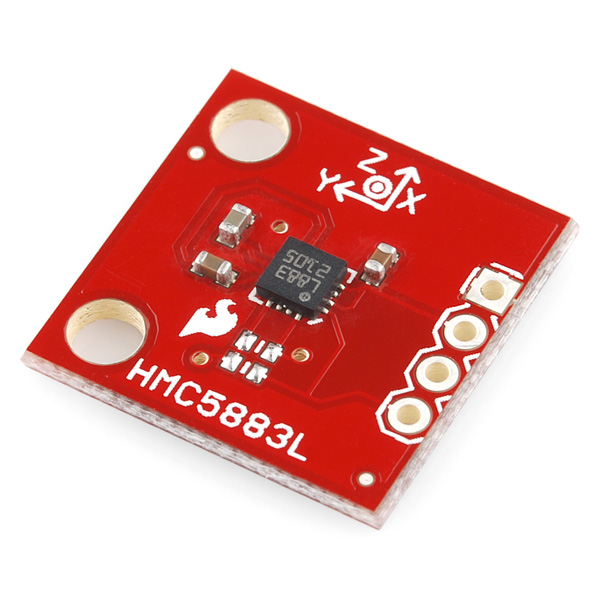
\includegraphics[width=0.6\textwidth]{figuras/5883L_BoB.jpg}
    \vspace{\baselineskip} %%% linha em branco para atender a norma
        \fonte{\cite{magnet}}
        \label{fig:magnetometro}
\end{figure}

Pode-se citar como principal vantagem o funcionamento em largas faixas de temperatura (entre -30°C e 85°C no caso do sensor mostrado acima) e também a alta confiabilidade das medidas. Entretanto, estes possuem uma área de sensibilidade baixa, o que leva ao problema anteriormente citado da necessidade de instalação de uma unidade por vaga.

Atualmente há algumas soluções no mercado baseadas em sensores magnéticos, como o PlacePod desenvolvido pela PNI Sensor, destacando-se a alta precisão na detecção dos veículos e a durabilidade de até 10 anos das baterias \cite{placepod}. Entretanto, o preço nada atrativo de U\$200 é um fator extremamente limitante, pois inviabiliza a escalabilidade desta solução. Há também empresas como a Libelium e a Paradox Engineering desenvolvendo produtos semelhantes, com precisão e durabilidade das bateriais semelhante, porém o preço destes não está disponível.

Além destes há o projeto de larga escala SFPark, iniciado em Abril de 2011 na cidade de São Francisco - CA, que foi implantado com o intuito de maximizar o número de vagas de estacionamento disponíveis. Para isso são utilizados em conjunto um sistema de detecção de veículos baseado em sensores magnéticos, com os parquímetros, afim de designar dinamicamente o preço das vagas conforme a disponibilidade, horário, e local. Dessa forma é possível saber em tempo real locais e preços de estacionamentos \cite{site:mobilize}.


\subsection{Sensores Ultrassônicos}
O princípio de funcionamento destes está relacionado à forma com que um sinal transmitido é refletido de volta ao entrar em contato com determinada superfície. Para tanto, pulsos de alta frequência são emitidos na direção do que se pretende analisar; depois a energia recebida de volta deve ser processada; e a partir disto é possível verificar, por exemplo, a que distância está um objeto ou também que tipo de material o elemento em questão é composto.

Dentre as vantagens preponderantes deste sensor está a praticidade de instalação e de se aferir resultados. Porém, diferentemente dos magnetômetros, situações climáticas adversas, como vento e chuva, causam perda de performance.

\subsection{Câmeras}
No caso destes sensores, a detecção das vagas de um estacionamento é feita através do uso de processamento de imagens. A alta capacidade de cobertura, ou seja, monitorar diversas vagas com apenas um só dispositivo, os tornam uma solução extremamente atrativa. Como pode ser visto na Figura \ref{fig:repoparking}, uma implementação de código aberto é capaz de detectar o estado de até quinze vagas de uma só vez.

\begin{figure}[H]
    \caption{\label{exepretex} Sistema \textit{Automatic Parking Detection} em operação}
    \centering
    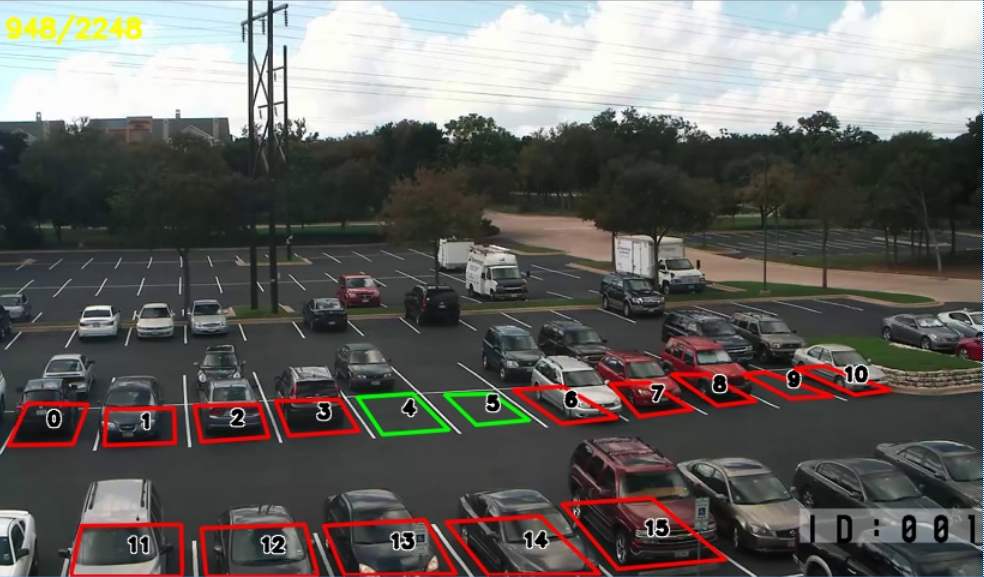
\includegraphics[width=0.6\textwidth]{figuras/automatic-parking-detection.png}
    \vspace{\baselineskip} %%% linha em branco para atender a norma
        \fonte{\cite{repoparking}}
        \label{fig:repoparking}
\end{figure}

\section{SENSORES DE LUMINOSIDADE LDR}
Como o nome sugere, estes dispositivos são capazes de medir a intensidade de luz em determinada região. Existem diversos tipos destes sensores, como fototransistores e fotoresistores, do inglês \textit{Light Dependent Resistor} (LDR), cada um produzindo medidas elétricas de uma forma. Por exemplo, no caso dos LDRs (geralmente representados como na Figura \ref{fig:ldr-simbolo}), a medida é realizada em relação à resistência interna destes, que varia de forma inversamente proporcional à incidência luminosa, comumente medida em Lux. A seguir são detalhadas as características dos fotoresistores.
\begin{figure}[ht]
    \caption{\label{exepretex} Simbologia de fotoresistores}
    \centering
    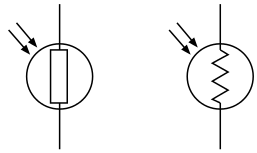
\includegraphics[width=0.6\textwidth]{figuras/ldrsymbol.png}
    \vspace{\baselineskip} %%% linha em branco para atender a norma
        \fonte{Adaptado de \cite{LightDep4:online}}
        \label{fig:ldr-simbolo}
\end{figure}


\subsection{Estrutura}
A estrutura dos fotoresistores é composta por uma trilha de algum material fotocondutor de alta resistência, como Sulfeto de Cádimo (CdS), conectada a terminais de contato de baixíssima resistência (Figura \ref{fig:ldrstructure}). Estes ficam dispostos sobre uma camada de substrato isolante, como cerâmica (Figura \ref{fig:substrato}). Vale ressaltar que o material semicondutor é dopado negativamente afim de se atingir um nível de condutividade capaz de diferenciar intensidades luminosas. Além disso, a região em volta dos contatos metálicos é dopada positivamente para evitar que estes influenciem nas medidas do sensor \cite{LightDep25:online}.

\begin{figure}[H]
    \caption{\label{exepretex} Estrutura básica de um LDR}
    \centering
    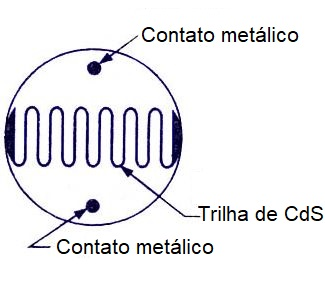
\includegraphics[width=0.6\textwidth]{figuras/ldrcds.jpg}
    \vspace{\baselineskip} %%% linha em branco para atender a norma
        \fonte{Adaptado de \cite{LightDep99:online}}
        \label{fig:ldrstructure}
\end{figure}

\begin{figure}[H]
    \caption{\label{exepretex} Camadas de um LDR}
    \centering
    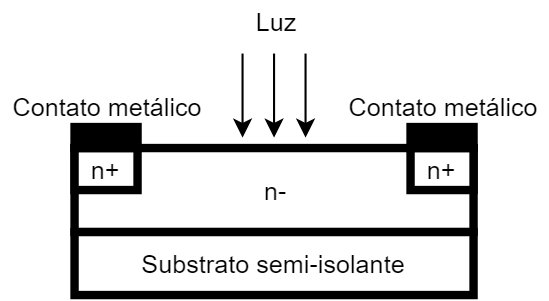
\includegraphics[width=0.6\textwidth]{figuras/ldr_esturtura.png}
    \vspace{\baselineskip} %%% linha em branco para atender a norma
        \fonte{Adaptado de \cite{LightDep25:online}}
        \label{fig:substrato}
\end{figure}

\subsection{Princípio de Funcionamento}
O funcionamento básico destes dispositivos consiste em variações na resistividade do material semicondutor que o compõe, conforme a intensidade luminosa incidente, e se dá através do efeito fotoelétrico,  postulado por Einsten em 1905 \cite{klassen2011photoelectric}. Isto é, quando a luz sobre o LDR for de alta frequência, os prótons absorvidos terão energia suficiente para fazer com que elétrons presos na camada de valência pulem para a camada de condução \cite{ibrahim2016automated}. Dessa forma, quando houver alta luminosidade incidente, haverão mais elétrons livres disponíveis para a condução de corrente elétrica (maior fotocondutividade), e portanto menor resistência do LDR.

Pode-se visualizar este comportamento na Figura \ref{fig:ldr-graph}. Em casos de alta luminosidade, como entre 10Lux e 100Lux, a resistência interna do material está na faixa de centenas de Ohms, e para cenários escuros, tem-se um aumento para a extensão de mega Ohms. Esta relação é descrita pela constante do LDR $\gamma$, que define a taxa de variação de resistência do LDR, em relação a um intervalo bem definido de variação luminosa:
\begin{equation}
    \gamma = log(\frac {R_{start}}{R_{end}}),
\end{equation}
onde $R_{start}$ e $R_{end}$ representam a resistência do LDR sob as intensidades luminosas que delimitam o intervalo, em Lux. Geralmente os fabricantes fornecem o valor desta característica, que comumente equivale a valores entre 0.6 e 0.8, para LDRs compostos por Sulfeto de Cádimo \cite{Lightdep67:online}. Além disso, é possível obter outra relação útil, que determina o valor de incidência luminosa, em Lux, a partir da constante $\gamma$:

\begin{equation}
    L = (\frac{R_{LDR}}{R_{escuro}})^\gamma ,
\end{equation}
tal que $L$ representa o valor da incidência luminosa que deseja-se medir, e $R_{LDR}$ é a resistência atual do dispositivo.

\begin{figure}[ht]
    \caption{\label{exepretex} Iluminância relacionada à fotoresistência}
    \centering
    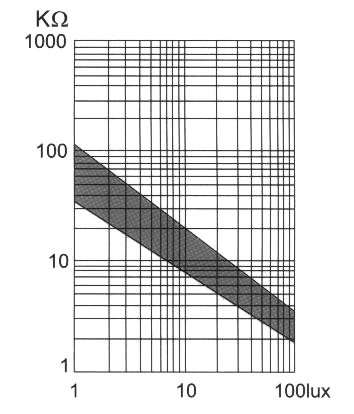
\includegraphics[width=0.6\textwidth]{figuras/ldrgraph.png}
    \vspace{\baselineskip} %%% linha em branco para atender a norma
        \fonte{Adaptado de \cite{noro2017common}}
        \label{fig:ldr-graph}
\end{figure}

% \subsubsection{Resposta Espectral}
Outro ponto relevante dos LDRs é a resposta espectral destes dispositivos. Similarmente ao olho humano, fotocondutores são sensíveis à determinada faixa de comprimentos de onda (cor da luz incidente). Portanto, o material utilizado para compor este tipo de sensor é determinante na curva de resposta espectral. Esta característica é muito importante, pois indica quais comprimentos de onda afetarão a resistência interna do dispositivo. A Figura \ref{fig:wavelength} exemplifica a operação de diferentes materiais sob a incidência luminosa. Pode ser observado que o Sulfeto de Cádimo (CdS) - amplamente utilizado em sensores LDR - opera principalmente na faixa de luz visível do espectro, sendo suficiente para a aplicação em questão, por se tratar da incidência de luz solar no sistema.
\begin{figure}[H]
    \caption{\label{exepretex} Resposta espectral de diferentes materiais}
    \centering
    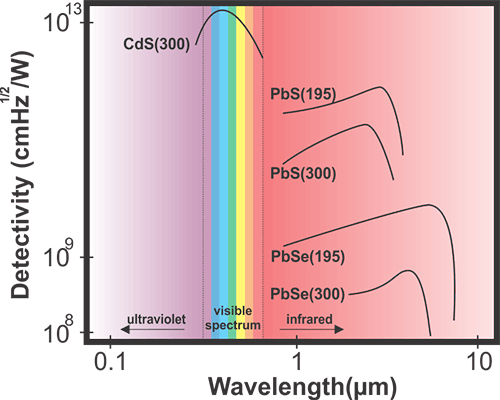
\includegraphics[width=0.6\textwidth]{figuras/wavelength-detectivity.png}
    \vspace{\baselineskip} %%% linha em branco para atender a norma
        \fonte{Adaptado de \cite{resistorguide}}
        \label{fig:wavelength}
\end{figure}



\chapter{REFERENCIAL TEÓRICO}
Este capítulo tem como objetivo abordar conceitos básicos relativos aos sistemas utilizados na aplicação proposta, como obtenção de medidas através de sensores analógicos e princípios de comunicação sem fio.

\section{REDES DE SENSORES SEM FIO}
Se há algo em comum entre todas as gerações humanas, pode-se dizer que isto é a curiosidade que temos de compreender o ambiente que nos circunda, e dar a isso algum valor. Dessa forma, diversos exemplos de aplicações, bem intencionadas ou não, que fossem baseadas na percepção ou monitoramento de eventos foram desenvolvidas ao longo dos anos. Na Segunda Guerra Mundial, por exemplo, a marinha alemã utilizava princípios eletromagnéticos para implantar minas navais que também atuavam como sensores, e assim eram capazes de afundar automaticamente navios britânicos quando próximos \cite{HowBrita11:online}. Em contrapartida, outros sistemas também antigos de percepção, como o radar são utilizados até hoje para fins mais pacíficos em áreas como meteorologia e aviação comercial. 

Com o passar do tempo, as técnicas de monitoramento foram aprimoradas e gradualmente mais automatizadas. Isto foi possível devido à rápida evolução na área de microeletrônica, que com circuitos e encapsulamentos cada vez menores e mais eficientes \cite{renna2007evolution}, possibilitou o surgimento das redes de sensores sem fio, que podem ser definidas como: sistemas compostos de nós sensores, que através de dispositivos perceptores juntamente com comunicação sem fio objetivam mensurar e transmitir informações sobre algum fenômeno. 

Nestas redes os nós sensores (\textit{sensor nodes}) são dispositivos de baixo consumo energético, equipados com sensores afim de detectar determinado evento, ou medida, de modo que a informação obtida seja transmitida por algum transceiver \cite{oliveira2011wireless}. Ou seja, por combinarem sensoriamento, processamento e comunicação em um só sistema, estes elementos são extremamente versáteis e possibilitam a criação de inúmeras aplicações. Entretanto ainda existem diversos desafios nesta área, como prolongar a vida útil das baterias, por exemplo. A seguir são apresentados alguns dos principais tópicos relevantes a estes sistemas.

\subsection{Visão geral}
Tipicamente redes de sensores sem fio (RSSFs) são definidas como um tipo especial de rede \textit{wireless}, onde cada nó trabalha cooperativamente para coletar e transmitir determinada informação \cite{loureiro2003redes}. Esta cooperação pode ser feita de diferentes formas, como por exemplo através da topologia de rede estrela (Figura \ref{fig:star-topology}), que consiste em nós independentes (\textit{sensor nodes}) enviando dados para uma central, usualmente chamada de \textit{sink node}, que os encaminha para outra rede, como a Internet, por exemplo \cite{buratti2009overview}. 
% DEFINIR OS TIPOS E ALGUMAS APLICAÇÕES

\begin{figure}[ht]
 	    \caption{\label{exepretex} Topologia estrela com \textit{sink-node} único}
    \centering
    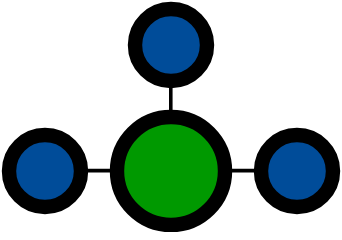
\includegraphics[width=0.6\textwidth]{figuras/star_topology.png}
    \vspace{\baselineskip} %%% linha em branco para atendender a norma
        \fonte{Autor (2018)}
        \label{fig:star-topology}
\end{figure}

Além do fator cooperativo entre os nós da rede, destacam-se alguns pontos cruciais que tornam estas redes diferentes do usual, como as limitações de energia que os \textit{sensor nodes} estão restritos, ou então a necessidade destes sistemas serem baratos, pois em muitas aplicações são utilizados inúmeros nós.

\subsection{Classificação e aplicações}
Pelas diversas possibilidades de aplicação destas redes, pode-se classifica-las de várias formas. Uma das mais utilizadas é a classificação baseada na topologia de rede, ou seja, como é estruturada a troca de informações entre os dispositivos participantes. Na Figura \ref{fig:topologias} são apresentadas algumas das topologias mais utilizadas em redes de sensores sem fio. 

\begin{figure}[ht]
 	    \caption{\label{exepretex} Topologias de rede}
    \centering
    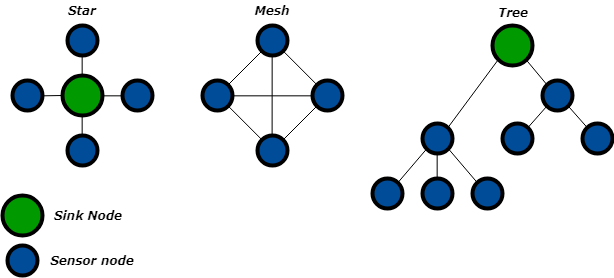
\includegraphics[width=0.8\textwidth]{figuras/toplogias.png}
    \vspace{\baselineskip} %%% linha em branco para atendender a norma
        \fonte{Autor (2018)}
        \label{fig:topologias}
\end{figure}

\begin{enumerate}
    \item Estrela (\textit{star}): Nesta topologia os \textit{sensor nodes} estão conectados a uma central (\textit{sink node}), também conhecida como nó coordenador ou mestre. Dessa forma, para que os \textit{sensor nodes} consigam trocar informações entre si, devem primeiro encaminhar os dados ao nó central. Dentre as principais vantagens de se utilizar esta estrutura de rede estão a simplicidade de implementação e o baixo consumo dos \textit{sensor nodes}. Entretanto, com apenas um nó coordenador há um ponto único de falha, e também maior consumo energético por parte deste.
    
    \item Malha (\textit{mesh}): Neste caso, todos os nós da rede que estejam próximos o suficiente podem trocar informações entre si, sem a necessidade de um nó coordenador. A complexidade dos nós, para que todos sejam capazes de rotear pacotes, por exemplo, torna estas redes não tão vantajosas para aplicações simples. Porém, caso a necessidade do sistema se concentre em alta tolerância a falhas e processamento distribuído, esta pode ser uma boa opção.
    
    \item Árvore (\textit{tree}): Já na topologia em árvore, os nós se comunicam através de uma hierarquia pré-definida. Isto é, os nós filhos, ou nós folha (\textit{leaf nodes}), de determinado nó, primeiro devem encaminhar seus dados ao nó pai para que cheguem ao avô, por exemplo. A principal vantagem de empregar esta topologia se concentra no baixo consumo dos nós filhos e alta escalabilidade. No entanto, quando um nodo pai tem algum problema, todos os \textit{leaf nodes} acabam sendo afetados, o que pode comprometer grande parte do sistema.   
    
\end{enumerate}

Além das topologias, também é possível classificar estas redes conforme o tipo de aplicação que são destinadas \cite{forster2016introduction}. Por exemplo, redes de sensores que coletem informações sobre o corpo humano são comumente chamadas de \textit{body sensor networks} \cite{espina2014network}. Dentre as aplicações mais comuns deste tipo de WSN encontram-se medições de pressão arterial; eletrocardiografia; ou até mesmo de movimento, através de sensores inerciais \cite{fortino2018wearable}.

Já redes implementadas para monitorar situações como a deste trabalho, isto é, com o intuito de obter dados do ambiente ou elementos deste, são nomeadas \textit{cyber-physical systems}, ou CPS. Neste caso destacam-se aplicações dispostas em áreas remotas, como o monitoramento de animais em migração \cite{zhang2004hardware}, ou então obtenção de dados de corais \cite{vasilescu2005data}, muito útil para biólogos. 

\subsection{Componentes}
Tipicamente estas redes consistem em dois sistemas básicos: nós da rede ou \textit{sensor nodes}, e central ou \textit{sink node}. 
Vale ressaltar que muitas vezes os \textit{sink nodes} não estão sujeitos às limitações energéticas inerente aos nós sensores, e dessa  forma consistem em apenas um computador diretamente conectado à rede elétrica, capaz de coletar e processar dados. Já os \textit{sensor nodes} são compostos pelos itens mostrados na Figura \ref{fig:sensor-node-components}, e devem ser selecionados criteriosamente, pois limitações como curta duração das baterias e precisão das medidas dos sensores impactam diretamente na aplicação. Abaixo são descritos brevemente estes sistemas.

\begin{figure}[ht]
 	    \caption{\label{exepretex} Componentes básicos de um \textit{sensor node}}
    \centering
    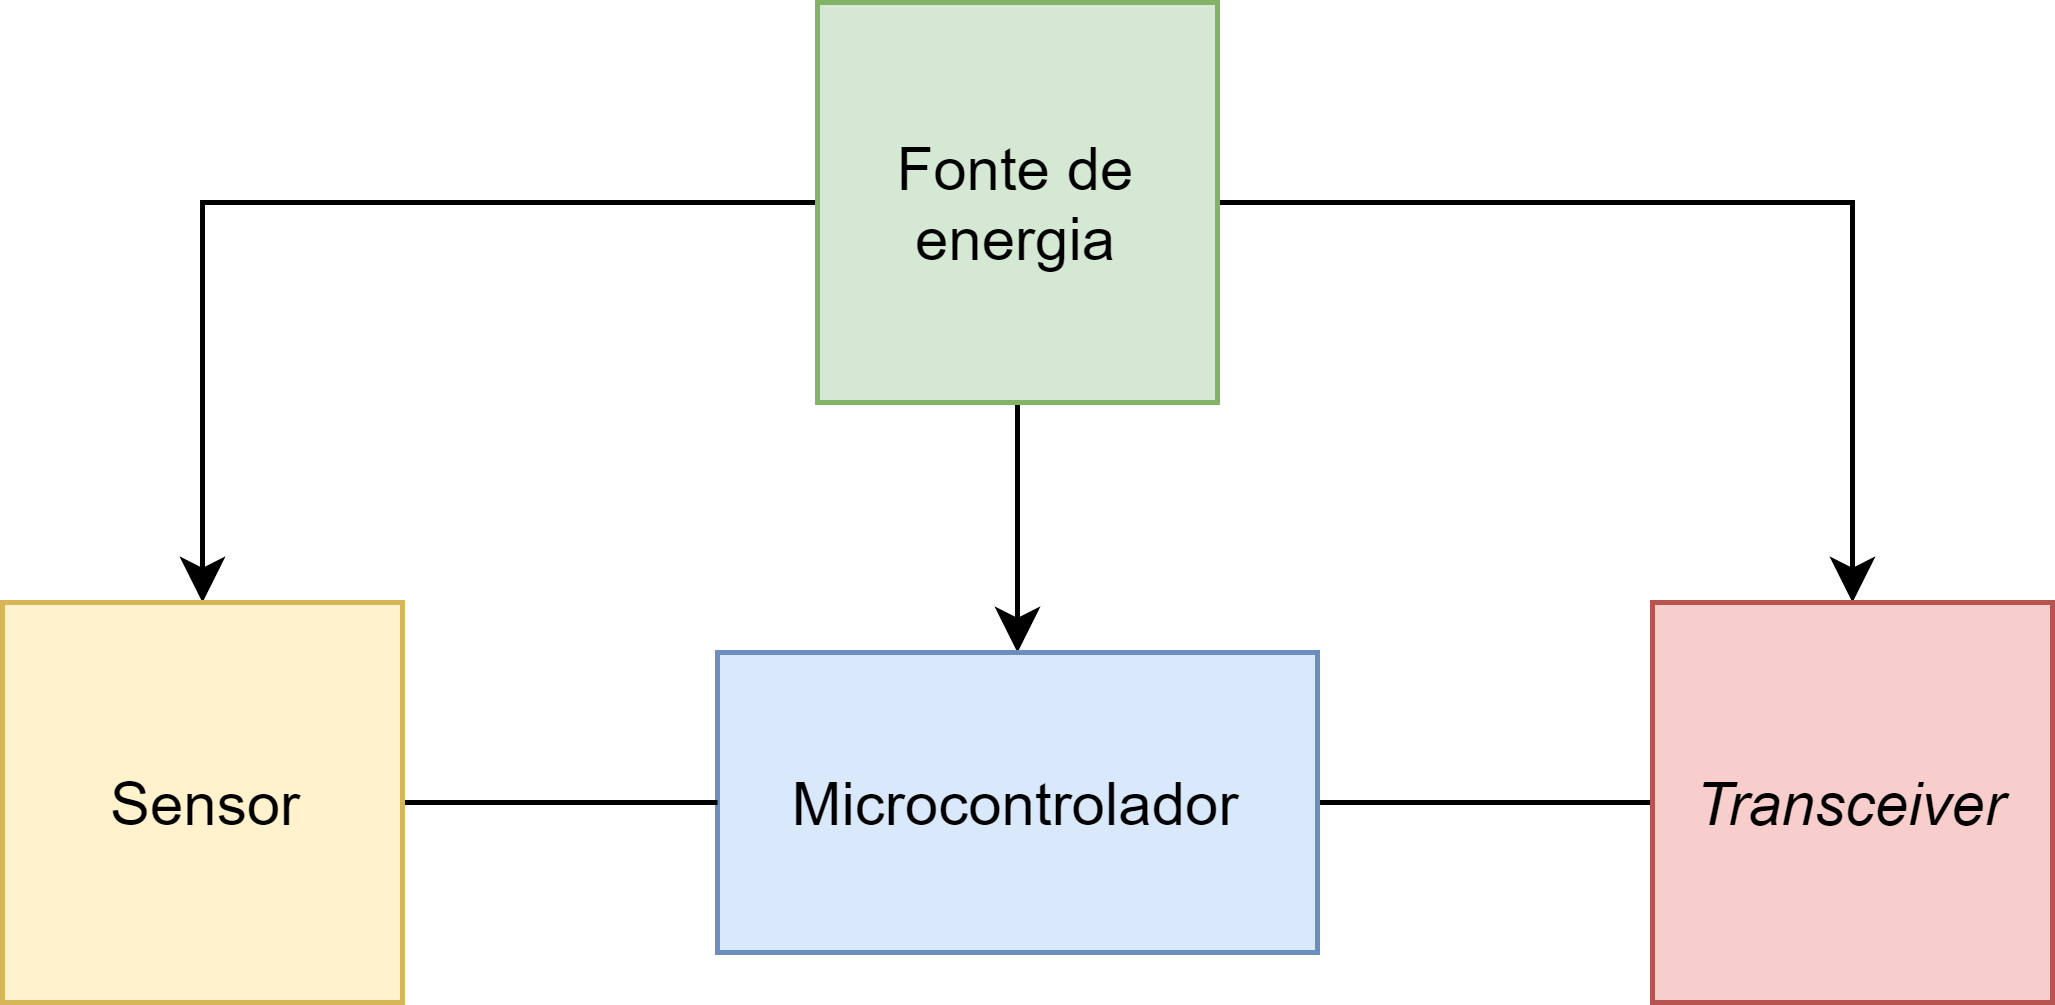
\includegraphics[width=0.6\textwidth]{figuras/wsn-blocks.png}
    \vspace{\baselineskip} %%% linha em branco para atendender a norma
        \fonte{Autor (2018)}
        \label{fig:sensor-node-components}
\end{figure}

\begin{enumerate}
    \item Fonte de energia: Para operar, estes sistemas necessitam de energia provida por pequenas baterias, como pilhas alcalinas ou baterias de lítio, por exemplo.
    \item Sensor: O elemento que dá nome aos nodos destas redes tem a função de mensurar alguma grandeza, ou evento, como a luminosidade em determinada região.
    \item Microcontrolador: Para tornar os dados dos sensores em algum útil são utilizados estes pequenos dispositivos, que já contém sistemas como processador e memória embutidos. Dentre as suas principais funções estão o processamento e interface com o dispositivo de transmissão.
    \item \textit{Transceiver}: Por fim, é necessário utilizar um transmissor \textit{wireless} para encaminhar as informações coletadas nos nodos. Geralmente estes dispositivos podem operar tanto como transmissores, quanto como receptores, sendo chamados de \textit{transceivers}.
\end{enumerate}

\subsection{Autonomia dos nós sensores}
Dentre as principais preocupações no desenvolvimento dos \textit{sensor nodes} encontra-se a longevidade e capacidade do sistema de alimentação empregado. Em uma aplicação composta por diversos nodos dispostos em uma área remota, como em plantações ou florestas, seria inviável utilizar baterias de curta duração, pois troca-las poderia acarretar em custos elevados. Portanto, é fundamental que a autonomia destes nodos seja devidamente projetada, levando em conta fatores como o consumo médio de cada dispositivo que compõe este sistema. Como mencionado em \cite{tan2013energy}, tipicamente os fatores mais relevantes para estimar a autonomia dos nós sensores são: 

\begin{itemize}
    \item Modo de operação: Este fator é extremamente importante, pois define o consumo médio necessário para realizar determinada ação. Em um sistema típico de WSN, deve-se considerar que a maior parte do tempo o sistema estará em modo de baixo consumo, e portanto exigirá menos da fonte de alimentação. Já quando estiver transmitindo dados, por exemplo, haverá um pico de consumo que será delimitante para o projeto.
    
    \item Tempo médio por operação: É essencial que se conheça o tempo necessário para realizar cada ação do sistema, pois este indica o quão impactante é o consumo em cada modo de operação. Usualmente é utilizada a técnica de \textit{duty cycling}, para prolongar a vida útil destes sistemas \cite{zhang2010energy}.
    
    \item Capacidade da bateria: Indica a máxima quantia de energia disponível da fonte de alimentação ao longo de um período de tempo. Geralmente esta informação é fornecida em mAh. 
\end{itemize}

% Com isso, relaciona-se estes parâmetros através de uma uma média ponderada:
% \begin{equation}
%     \overline{i} = \frac{1}{T_{ciclo}}\sum\limits_{n=1}^n [T_{n}(on)i_{n}(on) + T_{n}(off)i_{n}(off)],
% \end{equation}
% onde $\overline{i}$ representa o consumo médio total por ciclo de operação; $T_{ciclo}$ o tempo deste ciclo ($T_{on}$ + $T_{off}$); e $T_{n}$ e $i_{n}$ são o tempo e consumo médio necessários para realizar determinada operação $n$. Vale ressaltar que $on$ e $off$ se referem aos tempos de atividade e inatividade de cada dispositivo. Por exemplo, a transmissão de dados dos \textit{sensor nodes} não será contínua, portanto o tempo inativo ($T_{T}(off)$) será maior que o tempo em operação deste \textit{transceiver} ($T_{T}(on)$). Em um sistema que consista em 3 operações básicas, como a deste trabalho: leitura do sensor; processamento dos dados; e envio das informações, pode-se afirmar que o consumo médio será dado por:
% \begin{equation}
%     \overline{i}_{on} = \frac{T_{S}(on)i_{S}(on) + T_{M}(on)i_{M}(on) + T_{T}(on)i_{T}(on)}{T_{on}},
% \end{equation}
% \begin{equation}
%     \overline{i}_{off} = \frac{T_{S}(off)i_{S}(off) + T_{M}(off)i_{M}(off) + T_{T}(off)i_{T}(off)}{T_{off}},
% \end{equation}
% e finalmente:
% \begin{equation}
%     \overline{i} = \overline{i}_{on} + \overline{i}_{off},
% \end{equation}
% em que $\overline{i}$ é o consumo médio total por ciclo, dado em mA. Através dessa equação será estimada a necessidade de alimentação para o sistema. Vale ressaltar que geralmente as baterias contém informação de energia disponível por hora, como mAh, e por isso é interessante utilizar os tempos já convertidos em hora nos cálculos. Dessa forma, dado que uma bateria tenha uma capacidade de $i_{B}$ em mAh, então o tempo total de operação, em horas, de operação do \textit{sensor node} é estimado da seguinte forma:
% \begin{equation}\label{eq:time-of-operation}
%     n_{horas} = \frac{i_{B}}{\overline{i}}
% \end{equation}


\section{CONVERSÃO ANALÓGICO/DIGITAL}
Um dos procedimentos cruciais para este sistema proposto é a obtenção de dados do sensor de luminosidade, que consiste em converter os infinitos possíveis valores de tensão em algo palpável para a aplicação. Isto é, como a medida elétrica em questão se trata de um sinal contínuo no tempo, então deve-se transformar esta imensidão de possibilidades (sinal analógico) em uma informação compreensível para o controlador (sinal digital). Esta conversão é
feita por um circuito nomeado de conversor analógico/digital, também chamado de conversor A/D ou somente ADC, e consiste em algumas etapas (Figura \ref{fig:etapas-conversor}) detalhadas a seguir.

\begin{figure}[ht]
    \caption{\label{exepretex} Etapas para conversão analógico/digital}
    \centering
    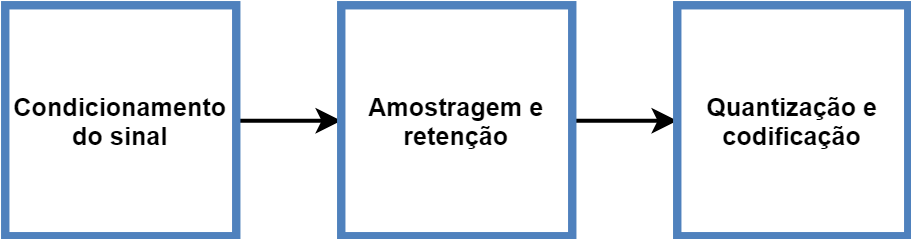
\includegraphics[width=0.6\textwidth]{figuras/conversor.png}
    \vspace{\baselineskip} %%% linha em branco para atender a norma
        \fonte{Autor (2018)}
        \label{fig:etapas-conversor}
\end{figure}

\subsection{Condicionamento do sinal}
Geralmente as medidas a serem convertidas são de faixas de tensão superiores ou inferiores à tensão de operação dos conversores A/D, que pode ser 3.3V ou 5V, por exemplo. Portanto, deve-se acomodar este sinal através de circuitos condicionadores, representados genericamente na Figura \ref{fig:condicionador-de-sinal-generico}.

\begin{figure}[ht]
    \caption{\label{exepretex} Condicionador de sinal genérico}
    \centering
    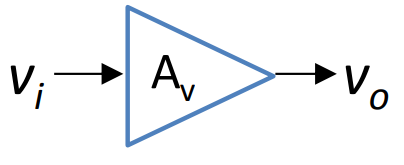
\includegraphics[width=0.6\textwidth]{figuras/condicionador-de-sinal.png}
    \vspace{\baselineskip} %%% linha em branco para atender a norma
        \fonte{Autor (2018)}
        \label{fig:condicionador-de-sinal-generico}
\end{figure}

Para que seja possível ler sinais da ordem de microvolts, como alguns sinais vitais de uma pessoa \cite{zhang2014signal}, por exemplo, é necessário amplificar este sinal de modo que seja compreensível para a aplicação em questão. Neste caso, o ganho $A_{v}$ deve seguir a relação abaixo: 

\begin{equation}\label{eq:condicionador-amplificador}
    |A_{v}| > 1,\quad \text{Ganho do condicionador para amplificação do sinal}    
\end{equation}

Já para casos em que o sinal a ser mensurado é de ordem de grandeza superior à do conversor, como equipamentos de alta de tensão, então utiliza-se o ganho situado na faixa da Equação \ref{eq:condicionador-atenuador}.

\begin{equation}\label{eq:condicionador-atenuador}
    0 < |A_{v}| < 1,\quad \text{Ganho do condicionador para atenuação do sinal}    
\end{equation}

Logo em sequência devem ser filtradas frequências que distorcem o sinal original a ser mensurado. Mais detalhes a respeito deste procedimento são descritos na próxima subseção.

\subsection{Amostragem e retenção}
Microcontroladores são capazes de operar com base em sinais digitais, ou seja, conjuntos de valores discretos no tempo que representem alguma grandeza, como textos e números inteiros. Entretanto, a grande maioria dos sinais presentes no universo são de natureza contínua e por isso devem ser discretizados para que sejam úteis a estes dispositivos eletrônicos. A discretização dos sinais analógicos já condicionados inicia através do processo de amostragem, que consiste em capturar de forma intervalada valores do sinal original, afim de se obter um conjunto finito de amostras que o represente.

Na Figura \ref{fig:processo-de-amostragem} é demonstrado o processo de amostragem baseado em uma série de impulsos, onde cada pulso é multiplicado pelo sinal original para se obter a amplitude deste naquele instante (representado pela Equação \ref{eq:amostragem}). 

\begin{figure}[ht]
    \caption{\label{exepretex} Processo de amostragem}
    \centering
    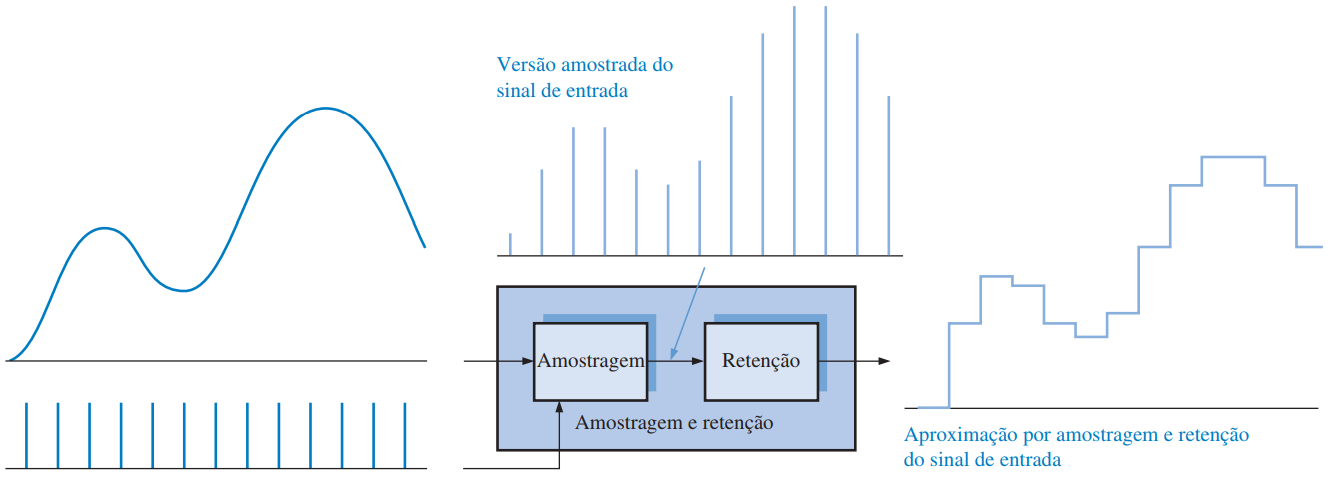
\includegraphics[width=0.8\textwidth]{figuras/sample-and-hold.png}
    \vspace{\baselineskip} %%% linha em branco para atender a norma
        \fonte{Adaptado de \cite{livro:sistemas-digitais}.}
        \label{fig:processo-de-amostragem}
\end{figure}

\begin{equation}\label{eq:amostragem}
    x_{d}(t) = \sum\limits_{n = -\infty}^\infty x_{c}(t)\delta(t-nT),
\end{equation}
onde $x_{c}(t)$ é o sinal a ser amostrado; $T$ define o período de amostragem;  $n$ é a ordem da amostra em determinado instante $t$; e $x_{d}(t)$ define o conjunto discreto de amostras, ou sinal discretizado \cite{livro:discrete-time-signal-processing}. O dispositivo responsável por este procedimento é popularmente conhecido como circuito de amostragem e retenção, do inglês \textit{sample and hold}, ou somente S/H.

Além disso, afim de se obter um sinal discretizado fidedigno ao original, deve ser cumprido o teorema da amostragem, formalmente postulado por Claude E. Shannon entre 1948 e 1949 \cite{luke1999origins}, que na prática determina que a frequência da função amostradora, trem de impulsos, por exemplo, deve ser pelo menos duas vezes maior do que a frequência do sinal a ser amostrado (Equação \ref{eq:teorema-amostragem}). 

\begin{equation}\label{eq:teorema-amostragem}
    f_{amostragem} \geq 2f_{sinal}
\end{equation}

Em outras palavras, a máxima frequência do sinal a ser amostrado deve ser inferior à metade da frequência de amostragem, mais conhecida como frequência de Nyquist (Equação \ref{eq:frequencia-nyquist}).

\begin{equation}\label{eq:frequencia-nyquist}
    f_{Nyquist} = 0.5f_{amostragem}
\end{equation}

Outro ponto relevante a ser considerado é o efeito de aliasing (Figura \ref{fig:efeito-aliasing}), que pode decorrer tanto do não cumprimento do teorema da amostragem, quanto das frequências harmônicas presentes no sinal original que possuem valor superior à frequência de Nyquist. Dessa forma, fica evidente que há a necessidade de filtragem destas frequências, pois amostrar um sinal distorcido provocará erros nas medidas discretizadas. Para isso pode ser utilizado um filtro passa-baixas, que eliminará apenas as frequências mais altas (Figura \ref{fig:passa-baixas}).

\begin{figure}[ht]
    \caption{\label{exepretex} Efeito de aliasing}
    \centering
    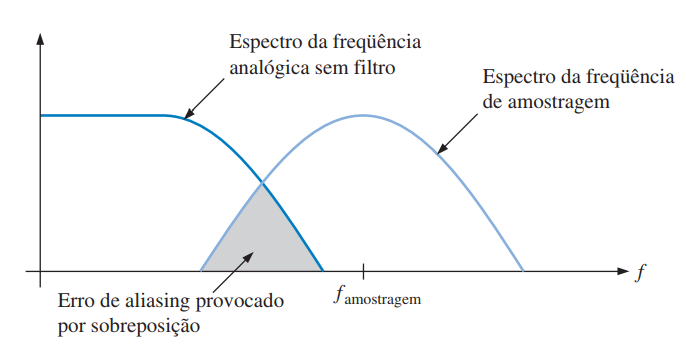
\includegraphics[width=0.8\textwidth]{figuras/aliasing.png}
    \vspace{\baselineskip} %%% linha em branco para atender a norma
        \fonte{Adaptado de \cite{livro:sistemas-digitais}.}
        \label{fig:efeito-aliasing}
\end{figure}

\begin{figure}[ht]
    \caption{\label{exepretex} Espectro do sinal filtrado por um passa-baixas}
    \centering
    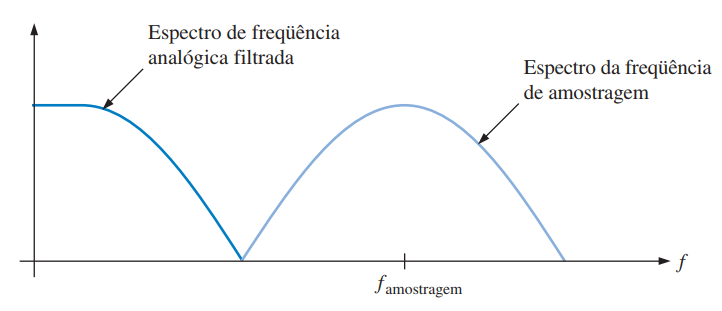
\includegraphics[width=0.8\textwidth]{figuras/passa-baixas.png}
    \vspace{\baselineskip} %%% linha em branco para atender a norma
        \fonte{Adaptado de \cite{livro:sistemas-digitais}.}
        \label{fig:passa-baixas}
\end{figure}

Vale ressaltar que o processo de filtragem faz parte do condicionamento do sinal, mas foi mencionado nesta subseção por decorrer dos parâmetros relevantes para amostragem.

\subsection{Quantização e codificação}
Após a discretização é realizado o processo de quantização, que consiste em converter as amostras obtidas do sinal original em valores que possam ser representados por uma quantidade finita de bits (sinal digital). Por exemplo, caso a resolução da quantização seja de 10 bits, como em \cite{ATmega3218:online}, então teoricamente pode-se mapear cada amostra em no máximo 1024 valores bem definidos, segundo a relação:

\begin{equation}
    N = 2^b,
\end{equation}
onde $b$ é a resolução do conversor, em bits, e $N$ é a quantidade de valores possíveis que podem representar uma amostra. Dessa forma, considerando um conversor de 5V e que seja quantizado e codificado uniformemente como no exemplo da Figura \ref{fig:quantizado-e-codificado}, tem-se:
\begin{flalign*}
    &N = 16\\
    &\Delta = \frac{5V}{16} \simeq 312.5mV
\end{flalign*}

Ou seja, neste caso a menor intensidade de tensão que o conversor pode codificar, conhecida como LSB, é de 312.5mV. Porém os valores entre 0 e 312.5mV, por exemplo, serão representados pelo mesmo símbolo e portanto serão medidas com erro de resolução. Este erro também é conhecido como erro de quantização, e pode chegar a no máximo $\pm$0.5LSB.

\begin{figure}[ht]
    \caption{\label{exepretex} Sinal quantizado e representado idealmente em codificação de 4 bits}
    \centering
    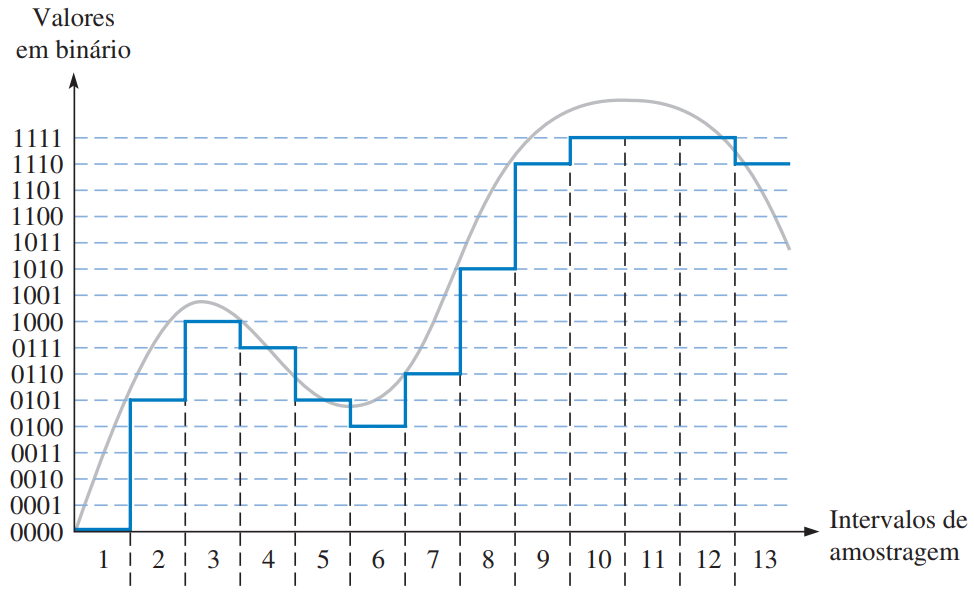
\includegraphics[width=0.8\textwidth]{figuras/quantizado-e-codificado.png}
    \vspace{\baselineskip} %%% linha em branco para atender a norma
        \fonte{Adaptado de \cite{livro:sistemas-digitais}.}
        \label{fig:quantizado-e-codificado}
\end{figure}

Com isso, é notável que a quantidade de bits disponível para a conversão A/D é um fator fundamental para obtenção de medidas confiáveis. Em uma aplicação que deseja-se uma resolução na ordem de pouquíssimos milivolts, como em exames de eletrocardiograma \cite{lopes2014processo}, por exemplo, a escolha do conversor deve ser meticulosa para atender esta necessidade.

Entretanto, além da resolução existem outros fatores limitantes à precisão destes conversores. Dentre estes aspectos destacam-se os erros estáticos (referentes a sinais DC), que são inerentes ao processo de quantização e podem ser classificados em quatro categorias detalhadas a seguir.

\begin{itemize}
    \item Erro de \textit{Offset}:
    Idealmente a curva que representa a quantização dos conversores A/D é tal que as transições entre o primeiro e o segundo código é realizada exatamente em $\pm$0.5LSB. Na prática isto não acontece (Figura \ref{fig:offset-adc}) e há sempre a possibilidade de ocorrer erro de \textit{offset}, definido como:
    \begin{equation}
        E_o = V_{tr} - V_{ti},
    \end{equation}
    onde $V_{tr}$ representa a tensão real da primeira transição de símbolo (de 000 para 001 em um conversor de 3 bits), e $V_{ti}$ a tensão de transição ideal (0.5LSB).  
    
    \begin{figure}[ht]
    \caption{\label{exepretex} Erro de \textit{offset}}
    \centering
    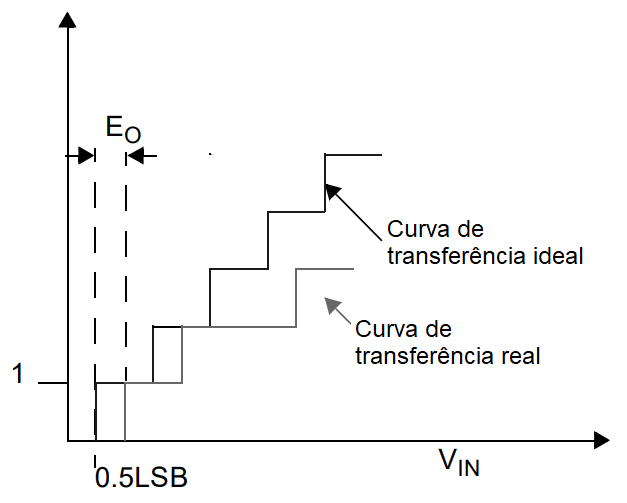
\includegraphics[width=0.6\textwidth]{figuras/erro_offset.png}
    \vspace{\baselineskip} %%% linha em branco para atender a norma
        \fonte{Adaptado de \cite{Understa51:online}.}
        \label{fig:offset-adc}
    \end{figure}
    
    \item Erro de ganho:
    Diferentemente do erro de \textit{offset}, o erro ganho está relacionado com a última transição de símbolo (de 110 para 111 para um ADC de 3 bits), e é representado por $Eg$ na Figura \ref{fig:eg-adc}.
    
    \begin{figure}[ht]
    \caption{\label{exepretex} Erro de ganho}
    \centering
    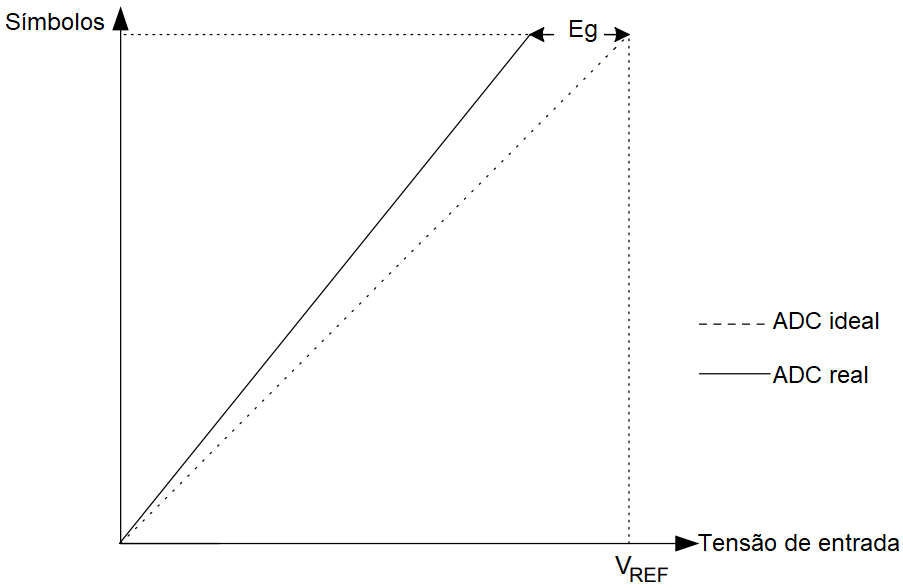
\includegraphics[width=0.8\textwidth]{figuras/erro_ganho.png}
    \vspace{\baselineskip} %%% linha em branco para atender a norma
        \fonte{Adaptado de \cite{ATmega3218:online}.}
        \label{fig:eg-adc}
    \end{figure}
    
    \item Erro de não linearidade diferencial (DNL):
    Este erro é definido como a máxima diferença entre as larguras real e ideal de cada código (000 por exemplo). Ou seja, a distância existente entre cada símbolo pode ser diferente de 1LSB, e é mensurado como mostra a Figura \ref{fig:dnl-adc}.
    
    \begin{figure}[H]
    \caption{\label{exepretex} Erro DNL}
    \centering
    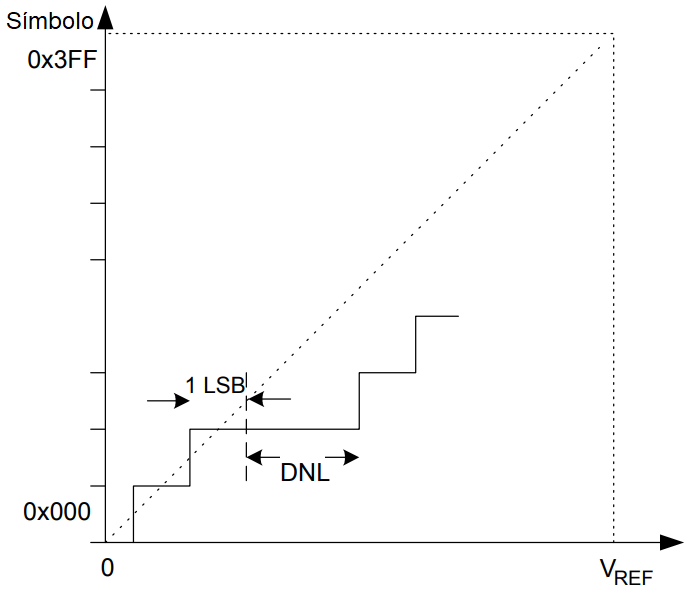
\includegraphics[width=0.8\textwidth]{figuras/erro_dnl.png}
    \vspace{\baselineskip} %%% linha em branco para atender a norma
        \fonte{Adaptado de \cite{ATmega3218:online}.}
        \label{fig:dnl-adc}
    \end{figure}
    
    \item Erro integral de não linearidade (INL):
    Assim como o DNL, este erro também decorre das limitações tecnológicas que tornam os conversores AD sistemas não lineares. Para determiná-lo, os fabricantes geralmente comparam a máxima distância vertical entre a curva de transferência real do ADC com a curva ideal de transferência deste dispositivo (Figura \ref{fig:inl-adc}).
    
    \begin{figure}[H]
    \caption{\label{exepretex} Erro INL}
    \centering
    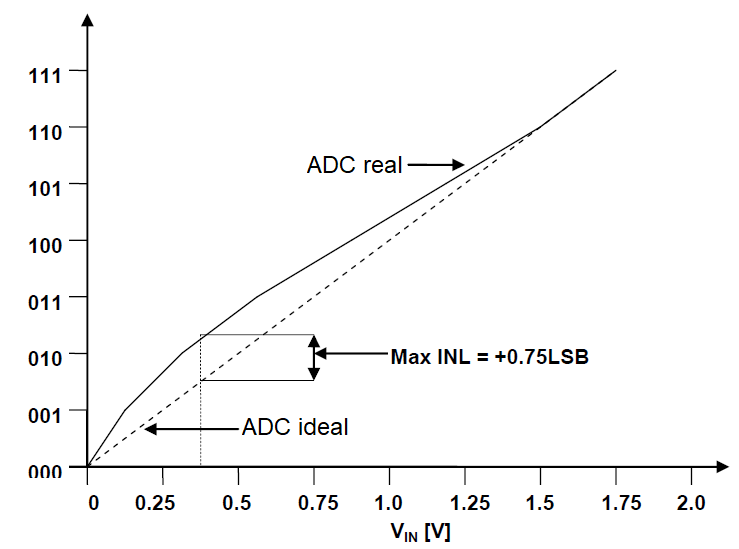
\includegraphics[width=0.8\textwidth]{figuras/adc-inl.png}
    \vspace{\baselineskip} %%% linha em branco para atender a norma
        \fonte{Adaptado de \cite{ADCInteg19:online}.}
        \label{fig:inl-adc}
    \end{figure}
\end{itemize}


\section{Comunicação por radiofrequência}
A etapa final necessária para os \textit{sensor nodes} de uma RSSF é a transmissão dos dados para a aplicação. Como mencionado anteriormente, geralmente utiliza-se um \textit{transceiver} operando em radiofrequência para este procedimento, que se baseia em alguns conceitos e etapas detalhadas a seguir.

\subsection{Radiofrequência}
Popularmente conhecidas como ondas de RF, as ondas de rádio ou radiofrequência são ondas eletromagnéticas com frequência delimitada no espectro de rádio (baixas frequências), como mostra a Figura \ref{fig:espectro}. Tipicamente os parâmetros que descrevem estas ondas são relacionados pela equação abaixo:
\begin{equation}
    y(t) = A(t)sin(2\pi f(t)t + \phi (t)),
\end{equation}

\begin{figure}[ht]
     \caption{\label{exepretex} Espectro eletromagnético para telecomunicações}
\centering
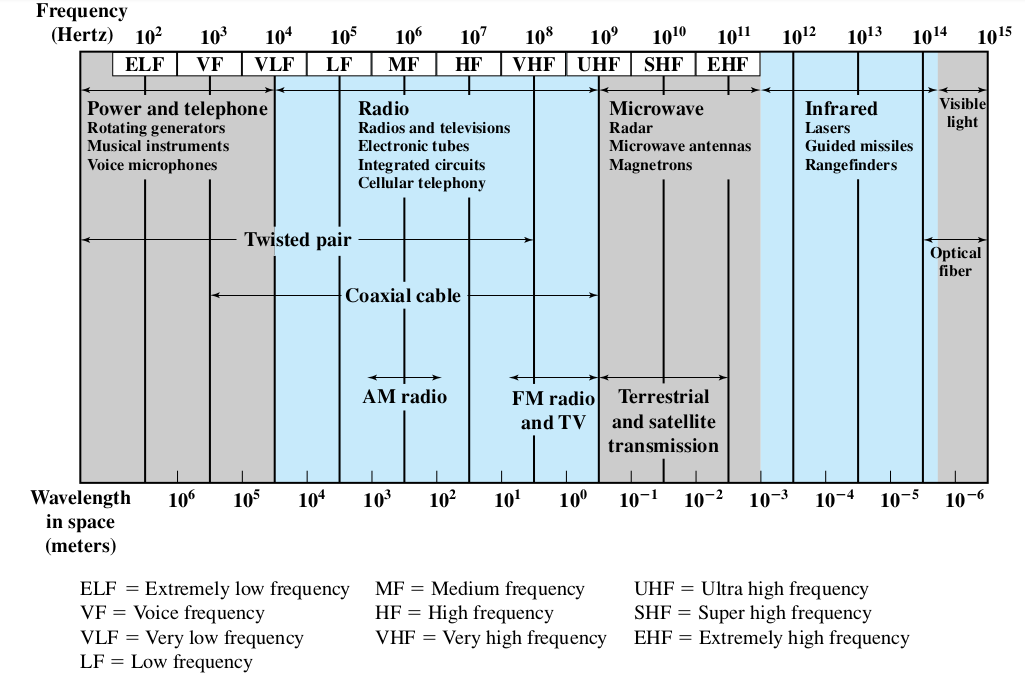
\includegraphics[width=0.8\textwidth]{figuras/espectro.png}
\vspace{\baselineskip} %%% linha em branco para atendender a norma
    \fonte{\cite{book:619676}.}
    \label{fig:espectro}
\end{figure}


onde $A(t)$ representa a amplitude desta função; $f(t)$ a frequência; e $\phi (t)$ a fase, ou desvio desta senoide com relação ao início dos eixos.

A partir disso, para que seja possível transmitir informações através destas ondas é necessário manipular os parâmetros que a descrevem, de forma que esta modificação seja perceptível tanto pelo transmissor, quanto pelo receptor. Isto é, assim como em uma conversa entre duas pessoas, é necessário que quem envia os dados (falante) fale o mesmo idioma que quem recebe (ouvinte). Este procedimento de manipulação sobre a onda em questão para inserção/recepção de informação é chamado de modulação/demodulação, e é descrito a seguir.

\subsection{Modulação}
Como mencionado anteriormente, o processo de modulação consiste em inserir informação em determinada onda, através da manipulação dos parâmetros que a descrevem. Por exemplo, em uma aplicação que transmita voz, como em estações de rádio, é necessário modular o sinal elétrico equivalente da fala em um sinal que possa ser transmitido pelo ar por longas distâncias. Para isso, é utilizado um sinal auxiliar, chamado de onda portadora, que tem o papel de sofrer variações em determinado parâmetro, como frequência ou amplitude, por exemplo, em função do sinal que deseja-se transmitir (sinal modulante). 

Além disso, deve-se ressaltar que as ondas portadoras são fundamentais neste processo, pois permitem que a transmissão de dados pelo ar seja possível sem a necessidade de antenas gigantescas. Isto é, como os sinais enviados se dão na forma de campos eletromagnéticos, então a máxima distância que determinado sinal poderá percorrer será delimitado pelo diâmetro da antena empregada para transmissão do campo \cite{book:1681103}.

% ABORDAR AM E MODULAÇÃO LORA
\subsection{Modulação digital AM}
Uma das técnicas de modulação digital mais simples empregadas em comunicação \textit{wireless} é a modulação ASK (\textit{Amplitude-Shift Keying}), que consiste em variar a amplitude de uma portadora conforme o sinal digital que deseja-se transmitir, de modo que a frequência e fase permaneçam constantes \cite{book:1039396}. Este tipo de modulação pode ser representado pelo diagrama de controle abaixo:
\begin{figure}[ht]
     \caption{\label{exepretex} Diagrama de controle de modulação ASK}
\centering
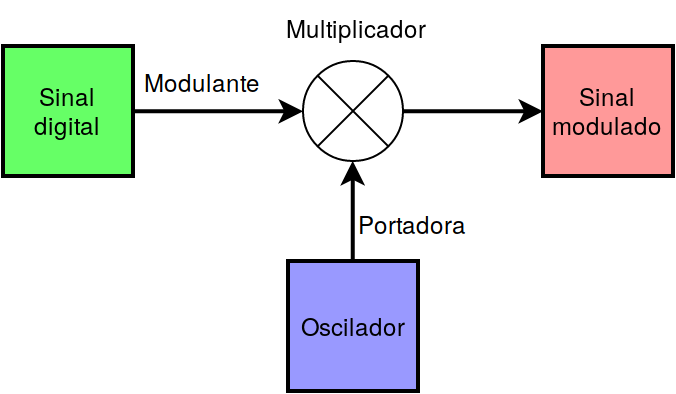
\includegraphics[width=0.6\textwidth]{figuras/ask-control.png}
\vspace{\baselineskip} %%% linha em branco para atendender a norma
    \fonte{Autor (2018)}
    \label{fig:ask-control}
\end{figure}

Tipicamente os bits do sinal de origem com valor 1 produzem as variações na amplitude da portadora, enquanto que os de valor 0 representam ausência de mudanças (Figura \ref{fig:modam}). 
\begin{figure}[ht]
     \caption{\label{exepretex} Sinal digital modulado/demodulado em amplitude}
\centering
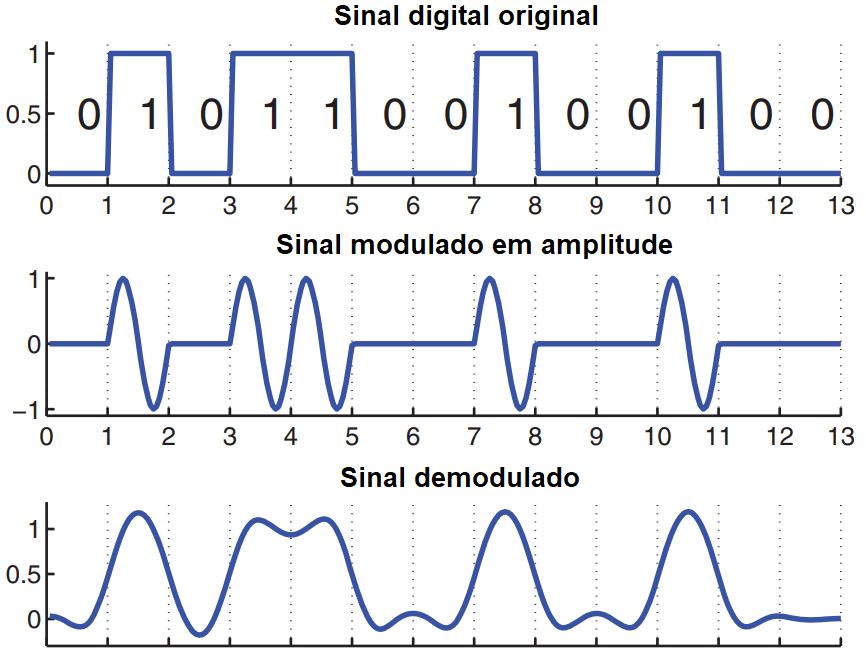
\includegraphics[width=0.6\textwidth]{figuras/modulacao.png}
\vspace{\baselineskip} %%% linha em branco para atendender a norma
    \fonte{Adaptado de \cite{puccinelli2005wireless}.}
    \label{fig:modam}
\end{figure}
Este procedimento pode ser descrito formalmente: dado um sinal digital a ser transmitido $d(t)$; sendo multiplicado por uma portadora $c(t)$; tem-se um sinal modulado $s(t)$ através da seguinte relação:
\begin{equation}
    s(t) = d(t)c(t),
\end{equation}
produzindo:
\begin{equation}
    s(t) =
\begin{cases}
    Acos(2\pi f_{c}t),& \text{sinal $d(t)$ em nível lógico 1}\\
    0,              & \text{sinal $d(t)$ em nível lógico 0},
\end{cases}
\end{equation}
onde $f_c$ é a frequência da portadora utilizada.

Vale ressaltar que a amplitude $A$ do sinal modulado é tipicamente representado na literatura, como em \cite{book:1681103} e \cite{book:1039396}, através da equação \ref{eq:amplitude}, que relaciona a amplitude RMS de uma senoide com a sua energia em função do tempo de bit $T$:
\begin{equation}\label{eq:amplitude}
    A = \sqrt{\frac{2E}{T}}
\end{equation}

% \subsection{Modulação por espalhamento espectral}

\section{LoRa}
A tecnologia de radiofrequência LoRa, criada pela empresa Semtech e desenvolvida atualmente pela LoRa Alliance, é caracterizada por possibilitar comunicação sem fio de baixo consumo e de longo alcance, sendo categorizada como uma LPWAN (\textit{low power wide area network}). Vale ressaltar que o termo LoRa se refere à camada física do sistema, enquanto que LoRaWAN ao protocolo de acesso ao meio (MAC) mais utilizado junto a esta tecnologia.

\subsection{Camada física}
A camada física LoRa foi desenvolvida pela Semtech e se caracteriza pela utilização da modulação \textit{Lora Spread Spectrum}, baseada na \textit{Chirp Spread Spectrum}, e pela operação nas bandas não licenciadas ISM (\textit{Industrial Scientific and Medical}). Nessa modulação a informação é codificada em \textit{chirps} (\textit{compressed high intensity radar pulses}) de frequência, que variam linearmente no tempo \cite{augustin2016study}. Para transmitir dados com esta técnica, inicialmente é enviada uma série de \textit{up-chirps} (\textit{preamble}) que delimitam o início de uma mensagem (\textit{payload}), como mostra a Figura \ref{fig:lora-message}. Vale ressaltar que o preâmbulo inicia com variações crescentes de frequência e termina com os chamados \textit{down-chirps}, que são variações decrescentes da mesma.

\begin{figure}[ht]
    \caption{\label{exepretex} Espectrograma de uma mensagem enviada por um transmissor LoRa}
    \centering
    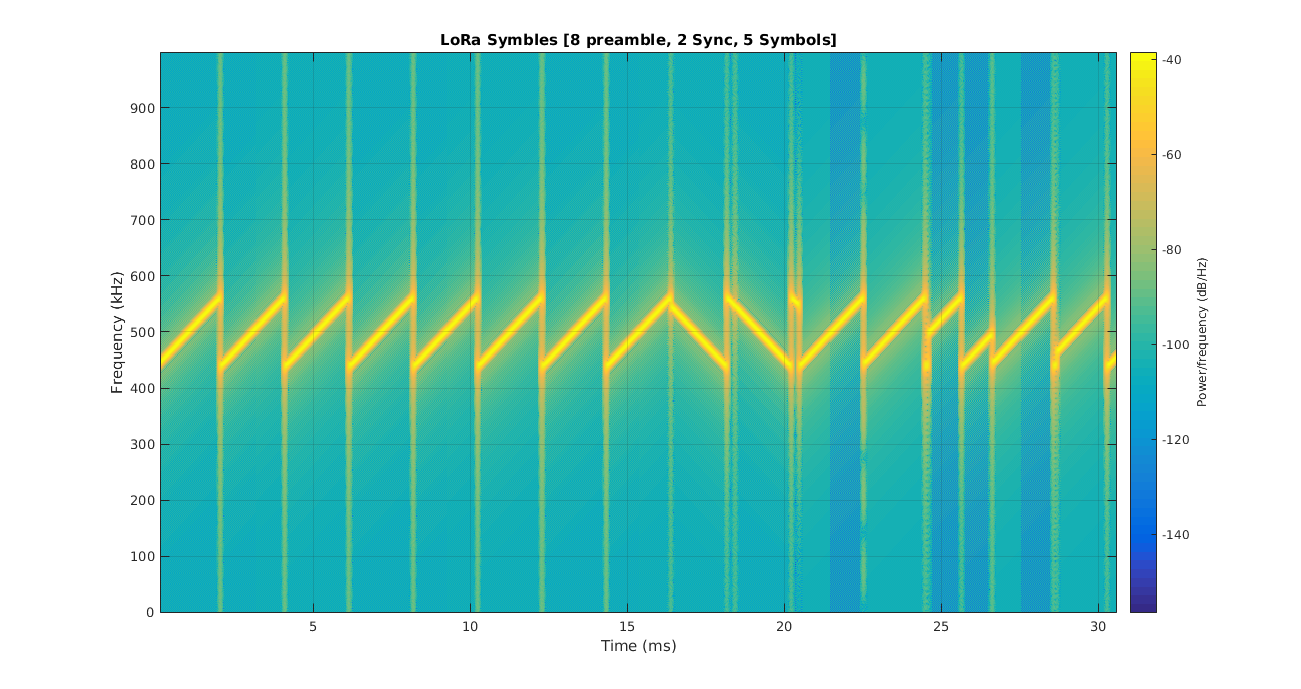
\includegraphics[width=0.8\textwidth]{figuras/lora-symbols.png}
    \vspace{\baselineskip} %%% linha em branco para atender a norma
        \fonte{\cite{lora-symbol-generation}.}
        \label{fig:lora-message}
\end{figure}

Dentre as principais vantagens de se utilizar esta modulação baseada em variações lineares de frequência estão a alta capacidade de transmissão com baixa potência, e também alta resistência ao efeito Doppler \cite{augustin2016study}.

\subsubsection{Parâmetros LoRa}
Dispositivos LoRa foram desenvolvidos de modo que possam operar com baixo consumo energético e transmissão de longo alcance. Para isso, é necessário que se configure tais dispositivos, ajustando os seguintes parâmetros:

\begin{enumerate}
    \item Largura de Banda (BW): Este parâmetro delimita a faixa de frequência utilizada pelos \textit{chirps} ao se transmitir dados. Variações neste fator afetam diretamente a taxa de transferência de dados e também a suscetibilidade da transmissão a ruídos. Tipicamente os valores de banda utilizados são de 125kHz, 250kHz e 500kHz.
    
    \item Fator de Espalhamento (SF): O fator de espalhamento define o quanto cada \textit{chirp} permanece ativo no tempo. Com isso, quanto maior o valor deste parâmetro, mais tempo cada \textit{chirp} estará espalhado no tempo, o que permite maior qualidade de transmissão em longas distâncias. Este fator pode ser configurado com valores entre 7 e 12 (Figura \ref{fig:lora-sf}). Visto que um símbolo LoRa é composto por $2^{SF}$ \textit{chirps}, então pode-se determinar a taxa de transmissão de dados, em bits por segundo, conforme \cite{lora-modulation-basics}:
    \begin{equation}
        R_b = SF\frac{1}{\frac{2^{SF}}{BW}}
    \end{equation}
    
    \begin{figure}[ht]
    \caption{\label{exepretex} Espectrograma de diferentes SFs}
    \centering
    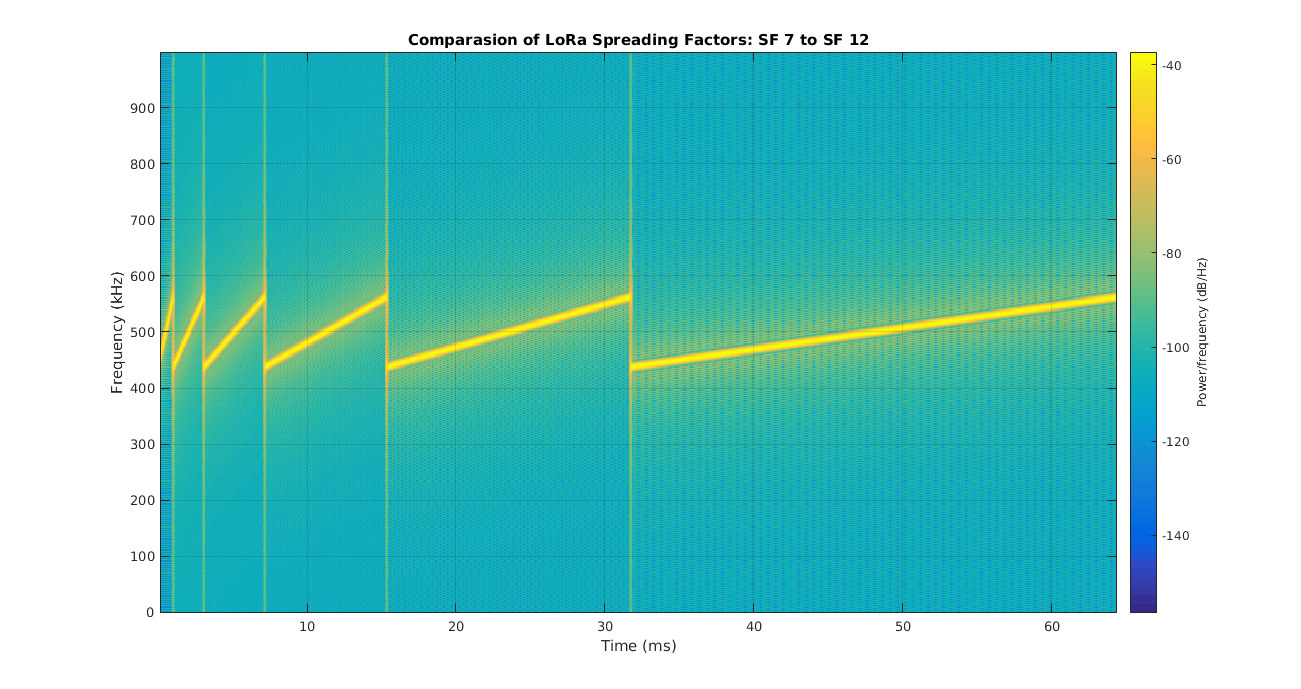
\includegraphics[width=0.8\textwidth]{figuras/lora-sf.png}
    \vspace{\baselineskip} %%% linha em branco para atender a norma
        \fonte{\cite{lora-symbol-generation}.}
        \label{fig:lora-sf}
    
    \end{figure}
    
    \item Taxa de Codificação (CR): Devido à técnica FEC (\textit{Forwared Error Correction}) de proteção contra interferências repentinas durante à transmissão de dados, dispositivos LoRa têm uma taxa de sobrecarga de redundância, chamada \textit{Coding Rate}, ou somente CR, que pode assumir os valores de 4/5, 4/6, 4/7 e 4/8.
\end{enumerate}

Além disso, existem os parâmetros regionais, como a frequência ou canal central de comunicação e potência máxima de transmissão, os quais são estabelecidos conforme as regulamentações de telecomunicações de cada país. No Brasil, por exemplo, rádios LoRa devem operar em torno da frequência de 915MHz, segundo a resolução nº 506 da Anatel \cite{ttn-frequencies}.

\subsection{LoRaWAN}
O protocolo de controle de acesso ao meio LoRaWAN, desenvolvido pela LoRa Alliance, possibilita utilizar as características da camada física LoRa em aplicações que necessitem longo alcance de transmissão, porém com baixa taxa de comunicação. Dentre os principais aspectos de redes LoRaWAN estão a independência entre dispositivos finais (\textit{end-devices}) e \textit{gateways}, e também a taxa de transmissão de dados adaptativa (\textit{Adaptative Data Rate}), que propicia uma forma de ajustar dinamicamente os parâmetros LoRa anteriormente citados.


\subsubsection{Arquitetura de rede}
\par
A arquitetura do sistema utiliza uma topologia estrela de estrelas, e é composta por quatro componentes, como mostra a Figura \ref{fig:lora-arch}.
\begin{figure}[H]
    \caption{\label{exepretex} Arquitetura LoRaWAN}
    \centering
    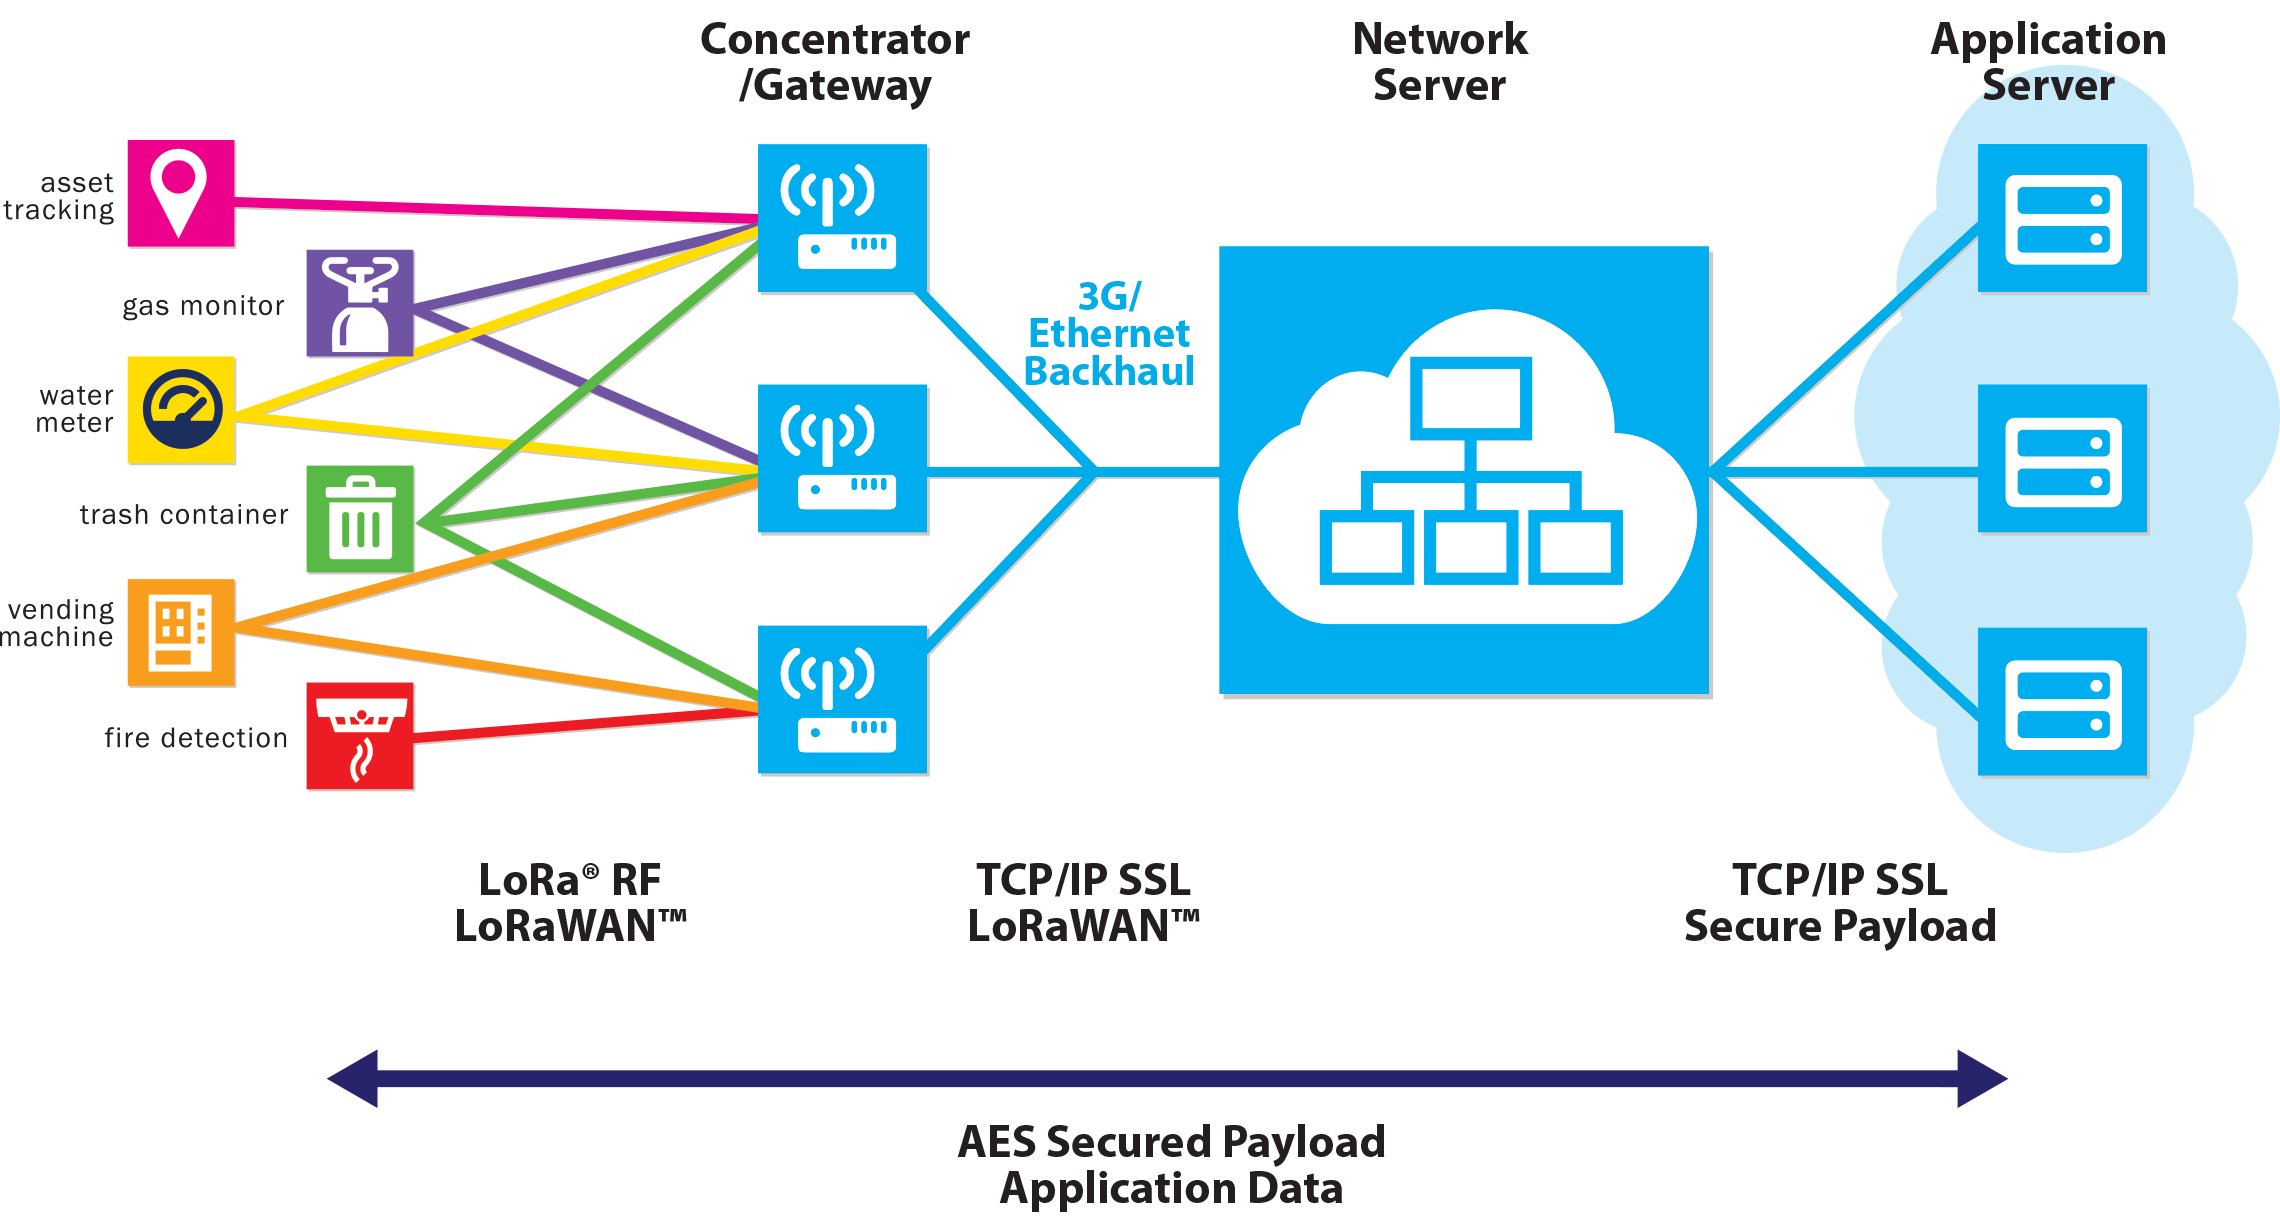
\includegraphics[width=0.8\textwidth]{figuras/what-network_diagram.png}
    \vspace{\baselineskip} %%% linha em branco para atender a norma
        \fonte{\cite{lora-arch}}
        \label{fig:lora-arch}
\end{figure}

\begin{enumerate}
    \item Módulos (\textit{end-devices}): Representam os sensores e atuadores conectados à rede via a interface de radiofrequência LoRa. Neste cenário, estes dispositivos transmitem dados sem destinatário em específico, o que os torna independentes dos \textit{gateways}. Vale ressaltar que estes podem operar de três formas diferentes, categorizadas como classes A, B e C, onde cada uma determina uma maneira de obter dados (\textit{downlink}) do servidor de rede.
    \item \textit{Gateways}: Também chamados de concentradores, estes são responsáveis pelo encaminhamento dos pacotes transmitidos pelos \textit{end-devices} aos servidores de rede. Atualmente o raio de cobertura destes fica entre 2km e 15km.
    \item Servidores de Rede: Estes são encarregados de filtrarem pacotes duplicados; realizarem controle de segurança e taxa de comunicação de dados (\textit{mac-commands}); envio de ACKs aos \textit{gateways}; direcionamento de pacotes para aplicações; em outras palavras, implementam toda a inteligência de rede necessária.
    \item Servidores de Aplicação: Estes servidores contém as aplicações em si. Tipicamente a obtenção de informações dos servidores de rede ocorre através de algum protocolo de comunicação de mensagens leves, como MQTT e CoAP.
\end{enumerate}

\subsubsection{Estrutura dos pacotes}
Mensagens de \textit{uplink} e \textit{downlink} são diferentes entre si, e são estruturadas como mostram os quadros \ref{uplink-msg} e \ref{downlink-msg}. Vale ressaltar que as mensagens de \textit{uplink} podem ser repassadas por mais de um \textit{gateway}, já que o tratamento de pacotes duplicados é feito pelos servidores de rede.

\begin{quadro}
   	    \caption{Mensagem de \textit{uplink}}
	    \centering
	    \begin{tabular}{| c | c | c | c | c |}
	    \hline
	    Preamble & PHDR & PHDR\_CRC & PHYPayload & CRC \\
	    \hline
	    \end{tabular}
	    \vspace{\baselineskip} %%% linha em branco para atendender a norma
	    \fonte{Adaptado de \cite{lorawan-specification}}
	    \label{uplink-msg}
\end{quadro}

\begin{quadro}
   	    \caption{Mensagem de \textit{downlink}}
	    \centering
	    \begin{tabular}{| c | c | c | c |}
	    \hline
	    Preamble & PHDR & PHDR\_CRC & PHYPayload \\
	    \hline
	    \end{tabular}
	    \vspace{\baselineskip} %%% linha em branco para atendender a norma
	    \fonte{Adaptado de \cite{lorawan-specification}}
	    \label{downlink-msg}
\end{quadro}

Nota-se que em ambos os tipos de mensagem há o preâmbulo (\textit{preamble}); LoRa \textit{physical header} (PHDR); \textit{header CRC} (PHDR\_CRC); e dados em si, ou \textit{payload} (PHYPayload). Entretanto apenas as mensagens de \textit{uplink} possuem proteção CRC, o que garante maior integridade dos dados enviados aos servidores de rede. Vale ressaltar que o campo de dados PHYPayload possui diferentes funções, como solicitação para entrada na rede ou envio de dados em si. Além disso, o identificador do dispositivo na rede é mantido no campo PHDR. A lista completa de informações sobre os pacotes LoRaWAN está disponível online em \cite{lorawan-specification}.


\subsubsection{Segurança}
A segurança em redes LoRaWAN é implementada em duas camadas: uma mantém a autenticação individual dos \textit{end-devices} na rede, e a outra garante que os dados dos dispositivos finais estejam protegidos \cite{lora-overview}. Para isso são utilizadas três chaves AES de 128 bits:  AppKey, NwkSKey e AppSKey. A primeira é utilizada para ativação dos dispositivos, tanto na forma OTAA (\textit{over-the-air activation}), quanto na ABP (\textit{activation-by-personalization}). O que diferencia estes dois modos de ativação é a maneira com que cada um gerencia as outras duas chaves, sendo que na ativação ABP os dispositivos ficam muito mais vulneráveis, pois dessa forma as chaves de criptografia de rede e aplicação (NwkSKey e AppSKey, respectivamente) ficam gravadas nos \textit{end-devices}.



\subsection{Protocolo MQTT}
Para obtenção de dados do servidor de rede são utilizados protocolos de conectividade entre dispositivos (M2M, do inglês \textit{Machine to Machine}). O protocolo \textit{Message Queue Telemetry Transport} (MQTT), originalmente desenvolvido pela IBM, é um destes, tendo como principal característica a utilização do paradigma \textit{publish}/\textit{subscribe} para troca de mensagens leves (Figura \ref{fig:mqtt-topico}).
\begin{figure}[H]
    \caption{\label{exepretex} Paradigma \textit{publish/subscribe}}
    \centering
    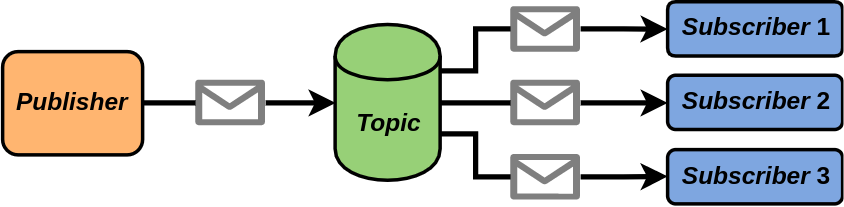
\includegraphics[width=0.8\textwidth]{figuras/publish-subscribe.png}
    \vspace{\baselineskip} %%% linha em branco para atender a norma
        \fonte{\cite{mqtt-diagram}}
        \label{fig:mqtt-topico}
\end{figure}

O funcionamento deste protocolo ocorre da seguinte forma: elementos que desejam receber algum dado de determinado tópico, se subscrevem a este; depois, a interface de comunicação, chamada de \textit{broker}, é responsável por gerenciar e encaminhar mensagens publicadas neste tópico. No caso de sistemas compostos por uma rede de sensores, por exemplo, os dados (\textit{payload}) são enviados para o gateway, sem distinção de tópicos neste momento; a partir disso, o gateway encaminha os dados ao servidor de rede afim de separá-los em tópicos relevantes, como "temperatura" ou "umidade do ar"; depois, alguma aplicação que deseja receber informações de temperatura, por exemplo, pode inscrever-se neste tópico; com isso, o \textit{broker} do servidor verifica os inscritos deste tópico, e os encaminha as mensagens publicadas pelos \textit{publishers}. 


\chapter{APLICAÇÃO DESENVOLVIDA}
Como mencionado nos capítulos anteriores, a busca às cegas por vagas de estacionamento disponíveis nas ruas é parcialmente responsável por problemas como congestionamentos e queimas desnecessárias de combustível. Partindo desta motivação, foi pensada e prototipada uma solução baseada em uma rede de sensores sem fio de baixo custo. 
Neste capítulo é descrito o sistema num todo, desde a definição dos componentes utilizados no projeto, até como é feita a transmissão dos dados.
    
    \section{VISÃO GERAL}
    Apesar de existirem algumas soluções no mercado para a informatização da disponibilidade de vagas de estacionamentos, geralmente as que se dão através de redes de sensores são caras, e portanto tornam-se inviáveis para um grande número de locais a serem monitorados. Dessa forma, o sistema proposto teve foco no uso de componentes de baixo custo e também na possibilidade de utiliza-lo em áreas remotas.
    
    Como pode ser visto na Figura \ref{fig:visao-geral}, o projeto é composto por cinco etapas. Na primeira é realizada a verificação do estado das vagas, através de sensores LDR independentes (\textit{sensor nodes}); depois, essa informação é propagada para o \textit{sink node} utilizando módulos de rádio AM; por sua vez, a central encaminha estes dados ao \textit{gateway} por intermédio de um rádio LoRa; diante disso o servidor de rede TTN obtém e disponibiliza o estado das vagas a um \textit{broker} MQTT; e por fim, comunicando-se com o \textit{broker} via MQTT a aplicação web disponibiliza estas informações.
    
    % e por fim, uma página disponibiliza estas informações utilizando comunicação via MQTT com o \textit{broker}.
    \begin{figure}[ht]
     	   \caption{\label{exepretex} Visão geral do sistema}
            \centering
            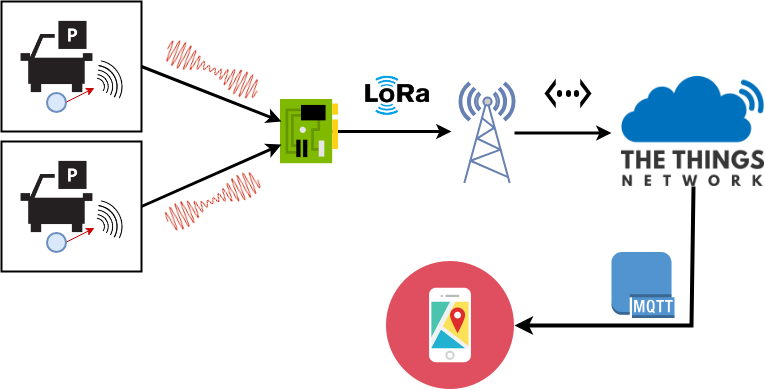
\includegraphics[width=0.8\textwidth]{figuras/funcionamento.png}
            \vspace{\baselineskip} %%% linha em branco para atendender a norma
                \fonte{Autor (2018)}
                \label{fig:visao-geral}
    \end{figure}
    
    A arquitetura de rede adotada consiste em uma rede estrela de estrelas, com duas camadas de comunicação sem fio. O motivo desta escolha se deu com o intuito de minimizar os custos da aplicação para que seja possível escalabilizar o sistema, isto é, para monitorar um número elevado de vagas, em diversos estacionamentos, é necessário que o preço unitário dos nós sensores seja baixo. Dessa forma, foram escolhidos módulos de rádio AM com um alcance razoável e de baixíssimo custo, de maneira que se utilize apenas um módulo LoRa (ainda muito caros no Brasil) para encaminhar o estado de várias vagas em determinado estacionamento. 
    
    
    \section{DESENVOLVIMENTO}
    O desenvolvimento desta aplicação foi dividido em três etapas: inicialmente foi realizado o projeto dos \textit{sensor nodes}, abrangendo desde o esquema elétrico à transmissão de pacotes; depois foi projetado o sistema \textit{sink node}, ou central; e por fim foi desenvolvida a aplicação que mostra a disponibilidade de vagas no local. A seguir são detalhados estes sistemas.
    
    \subsection{Projeto dos \textit{sensor nodes}}
    O projeto destes dispositivos foi feito com o objetivo de se ter um sistema barato capaz de informar o estado atual das vagas a cada 30 segundos, de modo que o consumo energético fosse reduzido ao máximo. Para isso, primeiramente foi estabelecido um fluxograma indicando cada etapa de operação deste sistema (Figura \ref{fig:flux-sensor-node}).
    
    \begin{figure}[ht]
     	    \caption{\label{exepretex} Fluxograma de operação dos \textit{sensor nodes}}
            \centering
            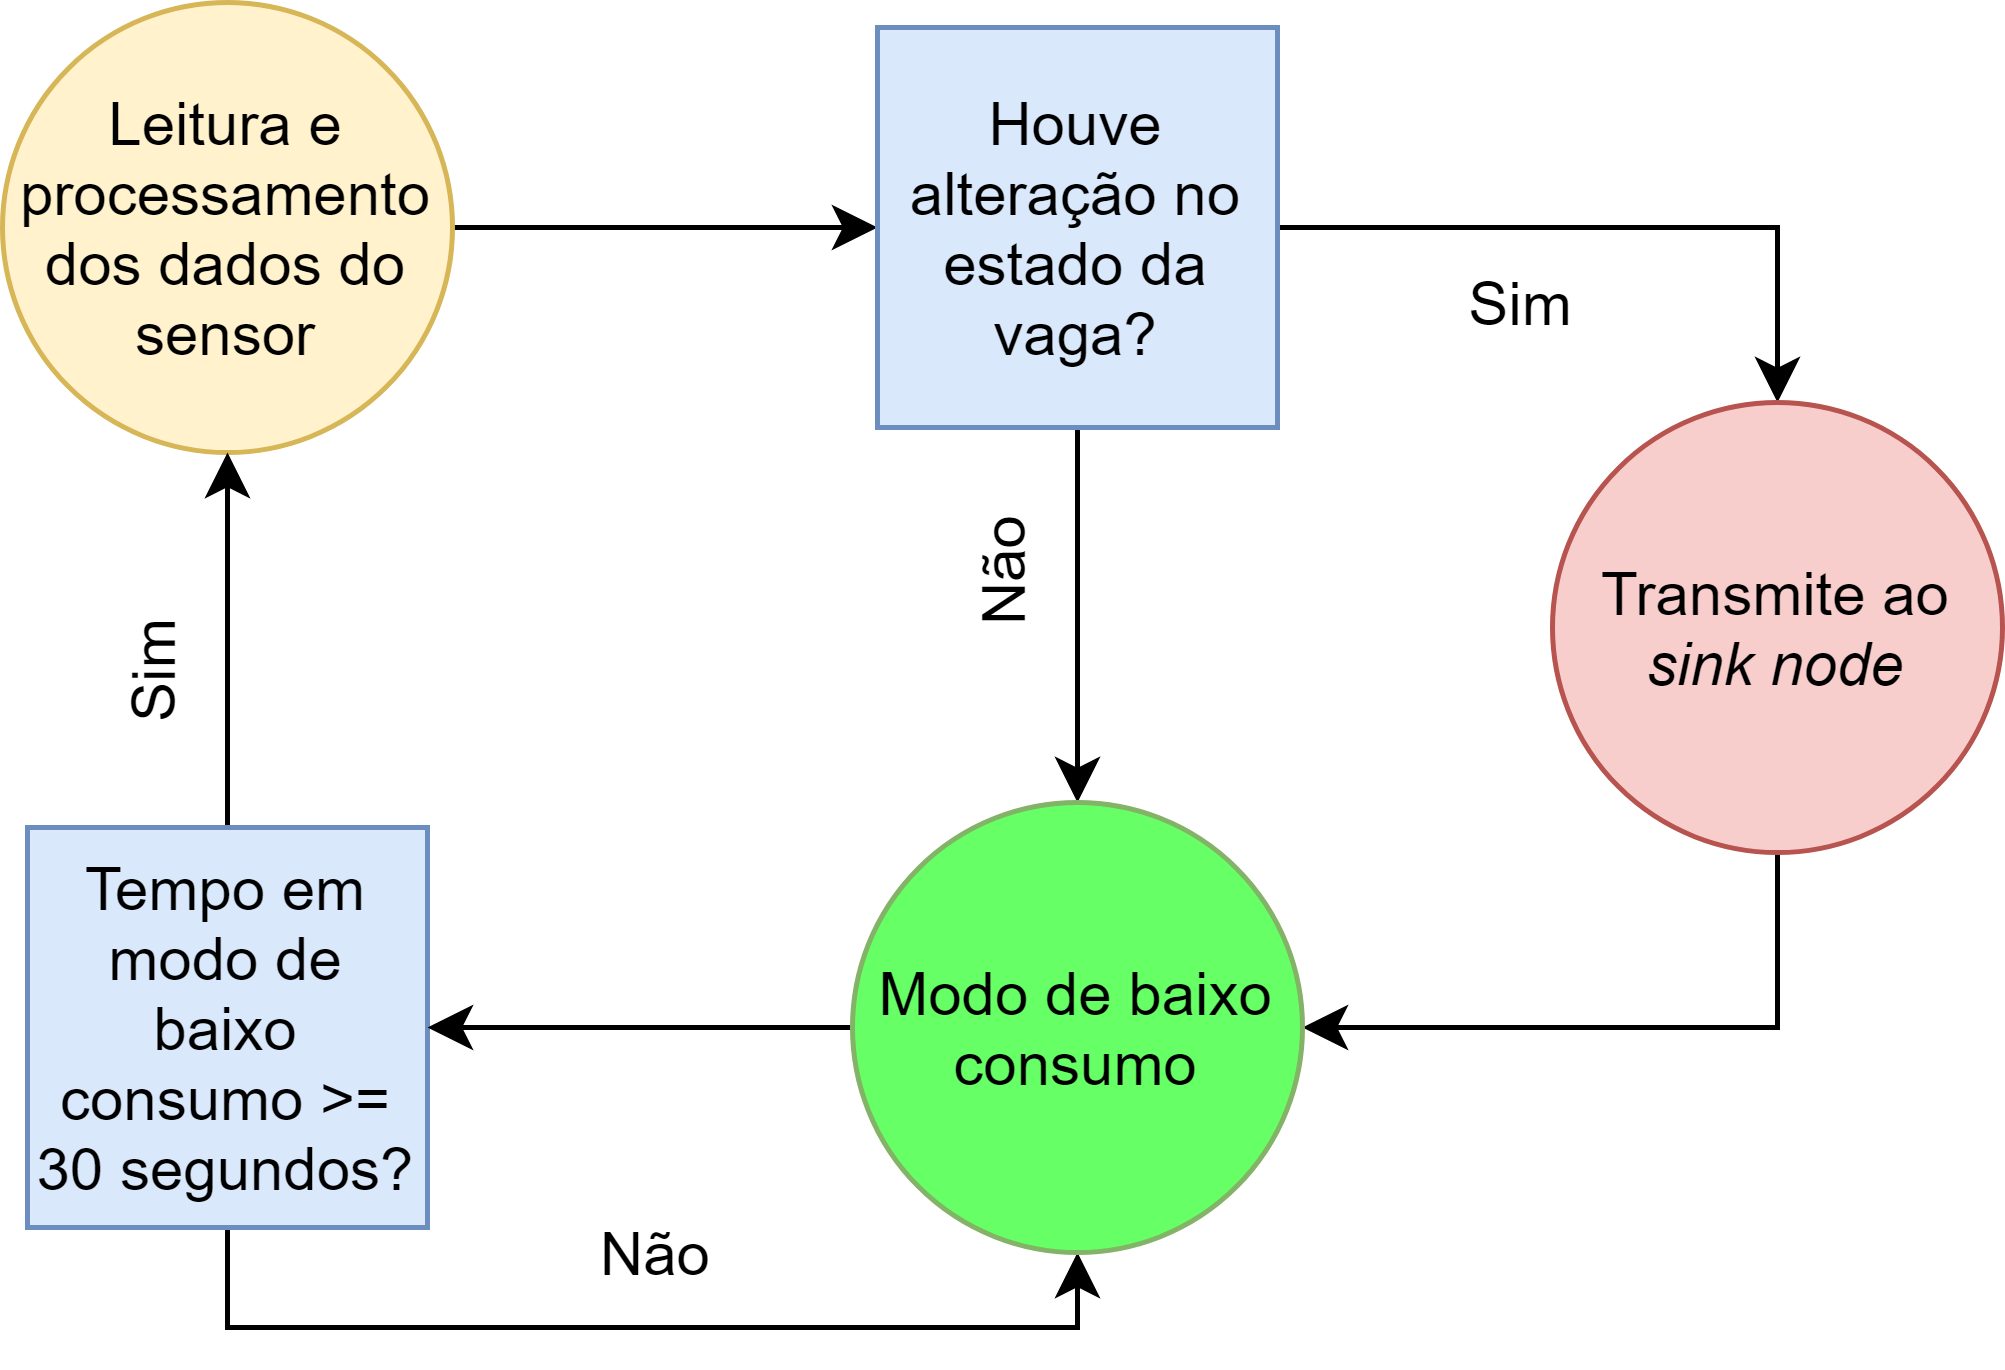
\includegraphics[width=0.6\textwidth]{figuras/sensor-node-fluxograma.png}
            \vspace{\baselineskip} %%% linha em branco para atendender a norma
                \fonte{Autor (2018)}
                \label{fig:flux-sensor-node}
    \end{figure}
    
    \begin{enumerate}
        \item Modo de baixo consumo (\textit{off}): Neste modo de operação o sistema mantém grande parte dos subsistemas desligados, como conversor AD e \textit{timers}, visando baixo consumo energético.
        \item Leitura do sensor e processamento dos dados do sensor: Nesta etapa são obtidas e analisadas amostras do sensor de luminosidade.
        \item Transmissão de dados: Caso haja mudança no estado da vaga, este dado é enviado ao \textit{sink node}.
    \end{enumerate}
    
    A partir disso foi feita a escolha dos componentes, visando baixo custo e baixo consumo energético.
    
    \subsubsection{Componentes}
    Tendo em vista a disponibilidade e praticidade para desenvolvimento deste sistema, foram utilizados os seguintes componentes de \textit{hardware}:
    \begin{itemize}
        \item Microcontrolador: ATmega328/P
        \item Sensor: LDR GL5528 
        \item Módulo RF: MX-FS-03V
        \item Bateria: 3 pilhas Duracell AA de 1.5V
        \item Resistor de \textit{pull-down}: 10k$\Omega$
    \end{itemize}
    
    Ainda que a escolha destes dispositivos tenha se concentrado em prolongar o tempo de duração das baterias, também foi necessário avaliar a robustez na obtenção de medidas por parte do circuito de sensoriamento. Isto é, o resistor de \textit{pull-down} teve de ser selecionado de modo que pequenas varições luminosas fossem percebidas, mas que também tivessem pouco impacto no consumo médio. Para isso, foram avaliados os seguintes resistores:
    
    \begin{table}[ht]
         \centering
         \caption{Avaliação do resistor de \textit{pull-down}}
         \begin{tabular}{ c c c }
             \hline
             Resistor [k$\Omega$] & Consumo máximo [$\mu A$] & Precisão [V] \\
             \hline
             10 & 250 & 0.0024 \\
             100 & 45 & 0.004 \\
             \hline
         \end{tabular}
         \vspace{\baselineskip} %%% linha em branco para atender a norma
          \fonte{Autor (2018)}
          \label{table:pull-down}
    \end{table}
    
    Dessa forma, ainda que o resistor de 10k$\Omega$ tenha um consumo teórico máximo cinco vezes maior que o de 100k$\Omega$, a precisão para casos de menor luminosidade é essencial para distinguir se determinada vaga está ou não ocupada, e portanto o seleciona para a aplicação.
    
    \subsubsection{Leitura do sensor}
    Nesta etapa é realizada a coleta de dados que indicam o estado atual das vagas. Para isso é utilizado o conversor A/D do microcontrolador, realizando medições do sensor LDR. Como pode ser visto no \textbf{ANEXO DO CÓDIGO DO SENSOR NODE}, é feita uma média de quinhentas medidas de luminosidade para aumentar a assertividade da presença ou não de um veículo no local.
    
    \subsubsection{Transmissão dos dados}
    Após a definição de presença ou ausência de veículo sobre a vaga, são enviadas mensagens com essa informação ao \textit{sink node}. Para tanto, foi empregado o módulo MX-FS-03V que opera em 315MHz e utiliza modulação ASK para comunicação de dados. Vale ressaltar que devido a este dispositivo ser apenas emissor, não é possível receber confirmação (ACK) de recebimento dos pacotes por parte da central. Após a transmissão do pacote o sistema volta ao modo de baixo consumo.
    
    \subsection{Projeto do \textit{sink node}}
    A central deste sistema foi projetada com o intuito de disponibilizar as informações recebidas dos \textit{sensor nodes} para a aplicação. Para encaminhar os dados à aplicação foi selecionada a tecnologia LoRa por dois motivos: aproveitar a disponibilidade de acesso a um \textit{gateway} já instalado sobre a reitoria da UFSM e também devido à capacidade de transmissão de dados em longas distâncias, permitindo que estacionamentos em áreas remotas, como em alguns lugares da universidade, pudessem ser monitorados sem a necessidade de roteadores, caso fosse utilizado Wi-Fi, por exemplo. Além disso, por utilizar uma faixa de frequência não licenciada, esta tecnologia se tornou ainda mais atrativa. E por fim, é possível expandir este sistema sem a necessidade de reprojetá-lo para comportar mais estacionamentos, vide a facilidade de se obter dados de dispositivos LoRa cadastrados na plataforma \textit{The Things Network}. A operação deste sistema está brevemente descrita no fluxograma da Figura \ref{fig:flux-sink-node}.
    
    \begin{figure}[ht]
     	    \caption{\label{exepretex} Fluxograma do \textit{sink node}}
            \centering
            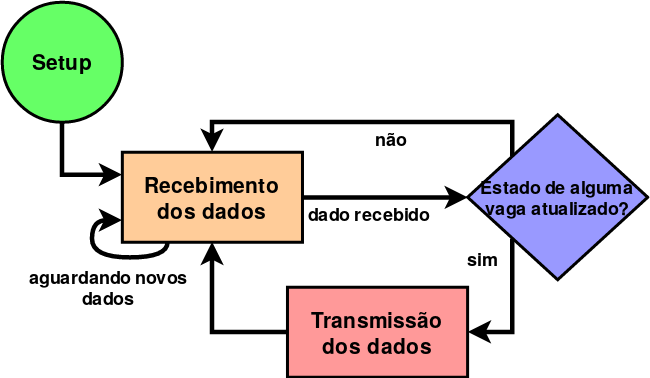
\includegraphics[width=0.6\textwidth]{figuras/central.png}
            \vspace{\baselineskip} %%% linha em branco para atendender a norma
                \fonte{Autor (2018)}
            \label{fig:flux-sink-node}
    \end{figure}
    
    \begin{enumerate}
        \item \textit{Setup}: Nesta etapa são definidas as configurações utilizadas no código.
        \item Recebimento dos dados: Este é \textit{loop} que aguarda dados dos nós sensores. 
        \item Estado de alguma vaga atualizado: Caso o estado de alguma das vagas tenha sido alterado, a central atualiza o número de vagas disponíveis.
        \item Transmissão dos dados: Finalmente a quantia de vagas disponíveis é enviada à aplicação.
    \end{enumerate}
    
    \subsubsection{Componentes}
    Foram utilizados os seguintes componentes de \textit{hardware}:
    \begin{itemize}
        \item Arduino Nano
        \item Recepetor AM MX-05V
        \item Módulo LoRa RFM95W
        \item Bateria de 9V
    \end{itemize}
 
    \subsubsection{Funcionamento}
    Como mencionado anteriormente, o sistema permanece em um \textit{loop} aguardando dados transmitidos pelos \textit{sensor nodes}.
    Assim como nos \textit{sensor nodes}, também foi utilizada a biblioteca RadioHead para recebimento dos dados. Quando chega uma nova informação, a central verifica com base no identificador do nodo remetente, se o estado da vaga em questão foi modificado, e então atualiza o contador de vagas disponíveis na área de cobertura do \textit{sink node}. Depois, é realizado o envio desta quantia, através da biblioteca LMIC, que implementa as funcionalidades necessárias para utilizar o protocolo LoRaWAN. O destinatário destas mensagens é um \textit{gateway} LoRa instalado na reitoria da Universidade Federal de Santa Maria, previamente testado e utilizado em \cite{tcc:matheus-neis}.
    
    
    \subsection{Aplicação final}
    A aplicação final do sistema consiste em dois subsistemas: \textit{backend} e \textit{frontend}. O primeiro é responsável por obter os dados do servidor de rede \textit{The Things Network} e encaminha-los ao servidor de aplicação, através do protocolo MQTT. Já o segundo busca as informações do servidor de aplicação, através de um cliente MQTT, e as mostra ao usuário.
    A seguir estão descritos estes dois subsistemas.
    
    \subsubsection{\textit{Back-end}}
    Inicialmente, foi definido o servidor de rede \textit{The Things Network} para ser usado na aplicação, pois o \textit{gateway} utilizado já estava vinculado ao sistema e também por ser prático na criação e gerenciamento de aplicações. Depois, foi desenvolvido um código na linguagem Python para obter em tempo real os dados do servidor. Para isso, foi utilizada a biblioteca de código aberto \textit{Eclipse Paho MQTT Python Client}, que oferece métodos de acesso através do protocolo MQTT. 
    
    \subsubsection{\textit{Front-end}}
    Neste módulo é apresentado quantas vagas estão disponíveis no estacionamento sob monitoramento. Para isso, foi desenvolvido um código em JavaScript que tem duas funções: obter os dados do \textit{backend}, utilizando a versão Javascript da mesma biblioteca \textit{opensource} \textit{Eclipse Paho MQTT}, e depois mostrá-los na tela. 
    
    \section{Implementação}
    A partir do projeto e definição de componentes foram prototipados os nós sensores e o nó central. Ambos foram previamente testados em \textit{protoboard} antes de serem montados nas placas de circuito impresso. 
    
    \subsection{Gravação de firmware no ATmega328P-PU via SPI}
    \textbf{TODO: Corrigir o esquemático - PINO de alimentação}
    Para programar o microcontrolador foi empregado um Arduino Nano configurado como gravador, conectando-o como mostra a Figura \ref{fig:gravador-sensor-node} e o quadro \ref{quadro:connections}. 
    
    \begin{figure}[ht]
 	    \caption{\label{exepretex} Diagrama de conexões entre gravador e microcontrolador}
        \centering
        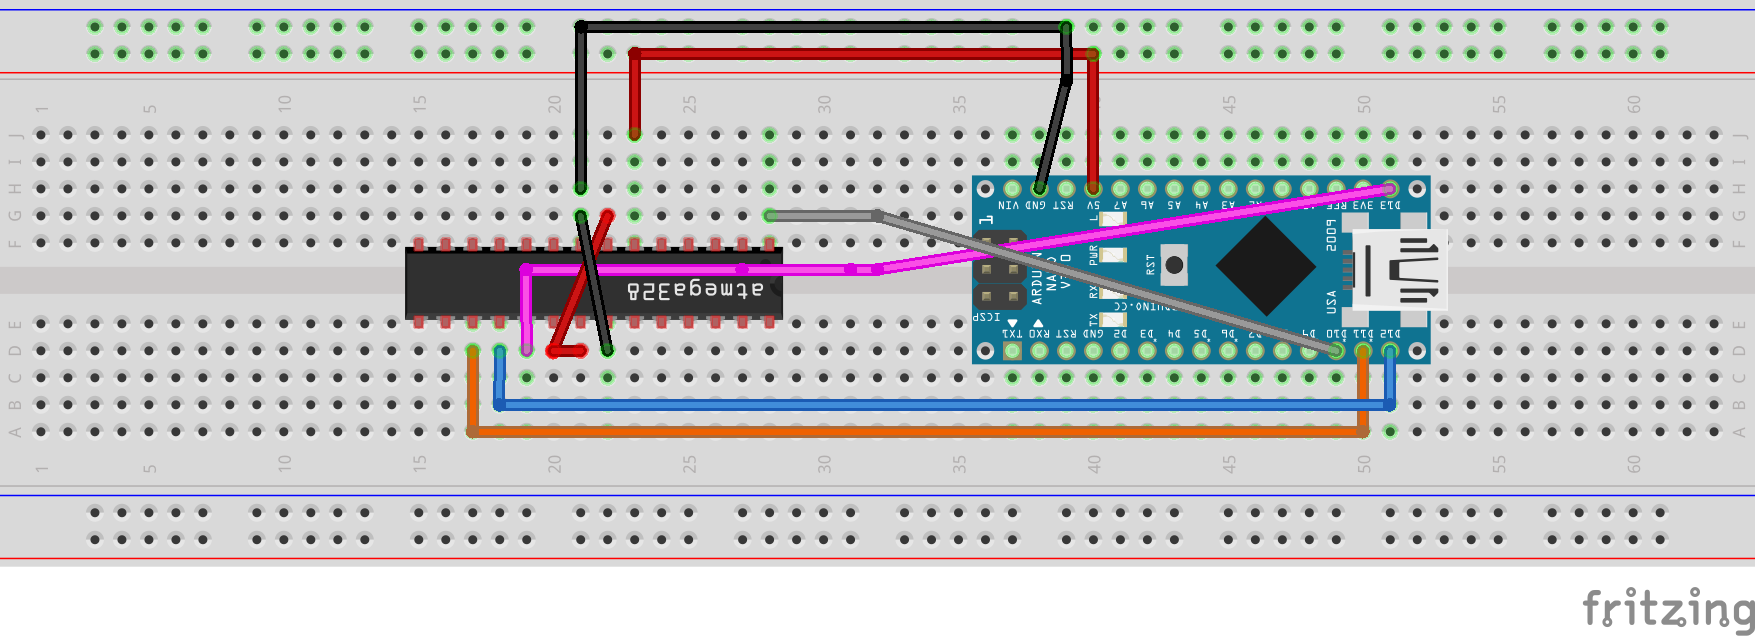
\includegraphics[width=0.8\textwidth]{figuras/firmware-programmer_bb.png}
        \vspace{\baselineskip} %%% linha em branco para atendender a norma
            \fonte{Autor (2018)}
        \label{fig:gravador-sensor-node}
    \end{figure}
    
    \begin{quadro}
   	    \caption{Conexões para gravação de \textit{firmware}}
	    \centering
	    \begin{tabular}{| c | c | c | }
	    \hline
	    Arduino Nano & ATmega328P-PU & Cor\\
	    \hline
	    5V & Pino 7 (VCC), Pino 20 (AVCC) e Pino 21 (AREF) & Vermelho\\
	    \hline
	    GND & Pino 8 (GND) e Pino 22 (GND) & Preto\\
	    \hline
	    D10 & Pino 1 (RESET) & Cinza\\
	    \hline
	    D11 & Pino 17 (MOSI) & Laranja\\
	    \hline
	    D12 & Pino 18 (MISO) & Azul\\
	    \hline
	    D13 & Pino 19 (SCK) & Rosa\\
	    \hline
	    \end{tabular}
	    \vspace{\baselineskip} %%% linha em branco para atendender a norma
	    \fonte{Autor (2018)}
	    \label{quadro:connections}
\end{quadro}
    
    As etapas para a gravação foram as seguintes:
    \begin{enumerate}
        \item Conectar o Arduino Nano ao computador, através de um cabo micro USB e na IDE do Arduino realizar o upload do \textit{sketch} "ArduinoISP", selecionando o \textit{programmer} "AVRISP mkll". Dessa forma a placa Nano se torna a interface de gravação.
        \item Depois, é necessário gravar o \textit{bootloader} no microcontrolador. Foi escolhido o \textit{bootloader} que utiliza a frequência de \textit{clock} interna de 8MHz do chip (disponível em \textbf{...}), por motivos de economia energética do nó sensor durante a operação. Para isso, primeiramente deve-se mover a pasta baixada para o diretório de \textit{sketches} da IDE do Arduino (no Windows geralmente se encontra em: C:/Users/user/Documents/Arduino). Depois, na IDE seleciona-se a placa "ATmega328 on a breadboard (8MHz internal clock)", configurando o \textit{programmer} "Arduino as ISP", e finalmente usar a ferramenta "Burn Bootloader".
        \item Por fim, deve-se abrir o código escrito para o \textit{sensor node} na IDE e fazer o \textit{upload} do mesmo através da ferramenta "Upload using programmer", disponível na seção ''Sketch'' do menu. Dessa forma, o microcontrolador estará pronto para operar.
    \end{enumerate}
    
    \subsection{Montagem}
    \textbf{TODO}: Com os \textit{firmwares} gravados
    
    \subsection{Gravação de \textit{firmware} no \textit{sink node}}
    \textbf{TODO}
    
    \subsection{Configuração do servidor de rede TTN}
    Nesta etapa é realizada a criação e configuração da interface de comunicação entre os dados vindos dos nós sensores, e a aplicação final. Dessa forma, primeiramente deve-se criar um usuário no sistema, e depois criar e configurar um dispositivo em ''Console'' na seção \textit{Applications} (Figura \ref{fig:add-app-ttn}). 
    
    \begin{figure}[ht]
 	    \caption{\label{exepretex} Criação de aplicação na TTN}
        \centering
        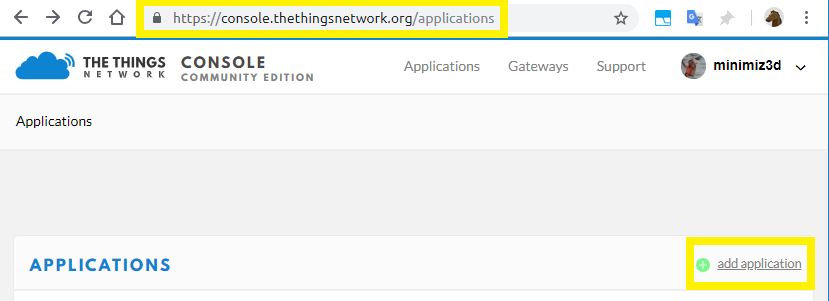
\includegraphics[width=0.8\textwidth]{figuras/teste.png}
        \vspace{\baselineskip} %%% linha em branco para atendender a norma
            \fonte{Autor (2018)}
        \label{fig:add-app-ttn}
    \end{figure}
    
    As configurações necessárias são as seguintes:
    
    \begin{enumerate}
        \item Quando criar um dispositivo, deve-se selecionar o \textit{handler} ''ttn-handler-brazil''.
        \item Depois, cria-se um \textit{device} com o identificador EUI gerado automaticamente, selecionando o botão destacado na Figura \ref{fig:dev-eui-ttn}.
        \item Com o dispositivo criado, deve-se navegar até o \textit{device} em questão na aba \textit{settings}, selecionando o método de ativação ABP (Figura \ref{fig:dev-settings-ttn}).
    \end{enumerate}
    
    \begin{figure}[ht]
 	    \caption{\label{exepretex} Seleção de EUI para dispositivo}
        \centering
        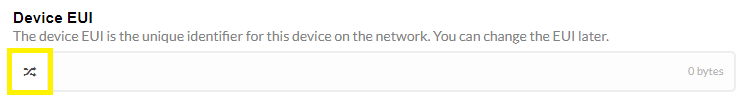
\includegraphics[width=0.8\textwidth]{figuras/device_eui.png}
        \vspace{\baselineskip} %%% linha em branco para atendender a norma
            \fonte{Autor (2018)}
        \label{fig:dev-eui-ttn}
    \end{figure}
    
    \begin{figure}[ht]
 	    \caption{\label{exepretex} Configuração do método de ativação ABP}
        \centering
        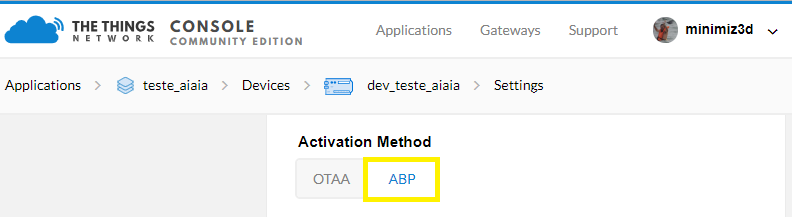
\includegraphics[width=0.8\textwidth]{figuras/device_settings.png}
        \vspace{\baselineskip} %%% linha em branco para atendender a norma
            \fonte{Autor (2018)}
        \label{fig:dev-settings-ttn}
    \end{figure}
    
    \subsection{Aplicação \textit{back-end}}
    Com as configurações da aplicação na TTN prontas, é necessário uma forma de obter e disponibilizar os dados enviados pelos sensores, recebidos e disponíveis no servidor de rede. Para isso, o código do \textit{backend} consiste em um cliente MQTT e um cliente \textit{MQTT over WebSocket}. O primeiro tem a função de obter continuamente os dados que chegam ao servidor de rede em determinado tópico (\textit{subscriber}). Já o segundo cliente tem o papel de \textit{publisher}, enviando os dados à aplicação de usuário (\textit{front-end}). Dessa forma, são necessários alguns parâmetros configurados na TTN, como chave de acesso (\textit{access key}), \textit{hostname} e a identificação ou nome da aplicação (\textit{Application ID}). O código utilizado na aplicação está disponível no Anexo \ref{}. 
    
    \subsection{Aplicação \textit{front-end}}
    Também chamada de aplicação final por ser o que é mostrado ao usuário, o \textit{front-end} tem a função de obter os dados fornecidos pelo \textit{back-end} e disponibilizar ao usuário de uma maneira agradável. No caso deste trabalho, esta aplicação consiste em duas partes: a primeira é responsável pela lógica de
    
    \section{Testes Realizados}
    Para avaliar a efetividade do sistema, foram testados isoladamente cada subsistema, como os sistemas de detecção e transmissão. Dessa forma, foi possível verificar primeiramente se os \textit{sensor nodes} realizam as medidas adequadamente no tempo esperado, e também se a comunicação, tanto dos nós para a central, quanto da central para o \textit{gateway} eram robustas para a aplicação. Por fim, com o sistema completo em operação, foram obtidos os resultados finais.
    
    \subsection{Autonomia}
    Primeiramente foi estimada a autonomia deste circuito, de modo que pudesse ser constatada a quantia de tempo que o sistema poderia operar sem a necessidade de substituir as baterias. Para isso foram obtidas medidas de tempo e consumo médio por modo de operação do sistema, da seguinte forma:
    
    \begin{enumerate}
        \item Medições de tempo: Para esta etapa foram desenvolvidos códigos que pudessem aproximar o tempo gasto em cada operação. 
        
        \item Medições de corrente: As medições do consumo médio se deram através de um multímetro em série com o circuito.
    \end{enumerate}
    
    Estas medidas, assim como a capacidade por modo de operação estão descritos na Tabela \ref{table:capacidade}. Vale ressaltar que estes valores de consumo médio por operação foram baseados no pior caso, ou seja, para casos de máximo consumo de corrente possível. Por exemplo, quando há muita luz incidente no sensor, este baixa sua resistência de modo que haja maior circulação de corrente pelo circuito, o que pode resultar em 250$\mu$A de consumo por parte do sensor (resistência mínima  de 10k$\Omega$ informada pelo fabricante).
    
    \begin{table}[ht]
         \centering
         \caption{Capacidade, tempo e consumo médio por modo de operação}
         \begin{tabular}{ l c c c }
             \hline
             Modo de operação & Tempo médio [s] & Consumo médio [mA] & \begin{tabular}{@{}c@{}}Consumo médio \\ por hora [mAh]\end{tabular} \\
             \hline
             Modo 1 (\textit{off}) & 30 & 0.0055 & 0.0021\\
             Modo 2 (sensor) & 0.055 & 6 & 7.64e-5\\
             Modo 3 (TX) & 0.450 & 13 & 0.0015\\
             \hline
              & Total: 30.505 & & Total: 0.0018
         \end{tabular}
         \vspace{\baselineskip} %%% linha em branco para atender a norma
          \fonte{Autor (2018)}
          \label{table:capacidade}
    \end{table}
    
    A medida de consumo médio por hora é necessária para determinar o tempo que o sistema poderá operar, visto que geralmente o dado fornecido por fabricantes de baterias é a capacidade ou energia disponível ao longo de uma hora (mAh). Portanto, estimando a quantia de energia média necessária para o circuito funcionar neste período, pode-se calcular a autonomia do circuito em diversas unidades, como horas de operação ou anos de operação. Estes valores estão presentes na Tabela \ref{table:autonomia} e são obtidos pelas relações abaixo:
    
    \begin{equation}
    n_{ciclos} = \frac{\text{Capacidade da bateria}}{\text{Consumo médio por hora}} = \frac{i_{bateria}}{i_{total}}
    \end{equation}

    \begin{equation}
        n_{horas} = \frac{n_{ciclos}}{(\frac{3600}{T_{total}})}
    \end{equation}
    
    \begin{equation}
        n_{dias} = \frac{n_{horas}}{24}
    \end{equation}

    \begin{equation}
        n_{meses} = \frac{n_{dias}}{30}
    \end{equation}
    
    \begin{equation}
        n_{anos} = \frac{n_{meses}}{12}
    \end{equation}

    \begin{table}[ht]
         \centering
         \caption{Autonomia teórica aproximada dos \textit{sensor nodes}}
         \begin{tabular}{ c c c c c }
             \hline
             Ciclos & Horas & Dias & Meses & Anos \\
             \hline
             1617021.2765 & 13702.0095 & 570.9171 & 19.0306 & 1.5859 \\
             \hline
         \end{tabular}
         \vspace{\baselineskip} %%% linha em branco para atender a norma
          \fonte{Autor (2018)}
          \label{table:autonomia}
    \end{table}
    
    \subsection{Medições do sensor LDR}
    Afim de verificar o quão precisas eram as medidas do sensor ao longo do dia, foram realizados testes no período das 8h às 18h, entre os dias 25, 26 e 28 de Setembro de 2018. Estes consistiram em colocar em operação um dos \textit{sensor nodes} no centro de 10 vagas, onde 5 destas estavam ocupadas, e as outras 5 livres, em um dos estacionamentos ao lado da Reitoria da UFSM. 
    
    \subsubsection{Testes de intensidade luminosa}
    Primeiramente foram obtidas medidas dos níveis de luminosidade sobre as vagas, afim de definir um valor de limiar (\textit{threshold}) que dita a presença ou ausência de veículos. Neste caso, foi utilizado um led em conjunto com o circuito original para indicar o nível de luminosidade sobre determinado local (Figura \ref{fig:led-indicator}).
    
    \begin{figure}[H]
     	    \caption{\label{exepretex} Circuito indicador de intensidade luminosa}
            \centering
            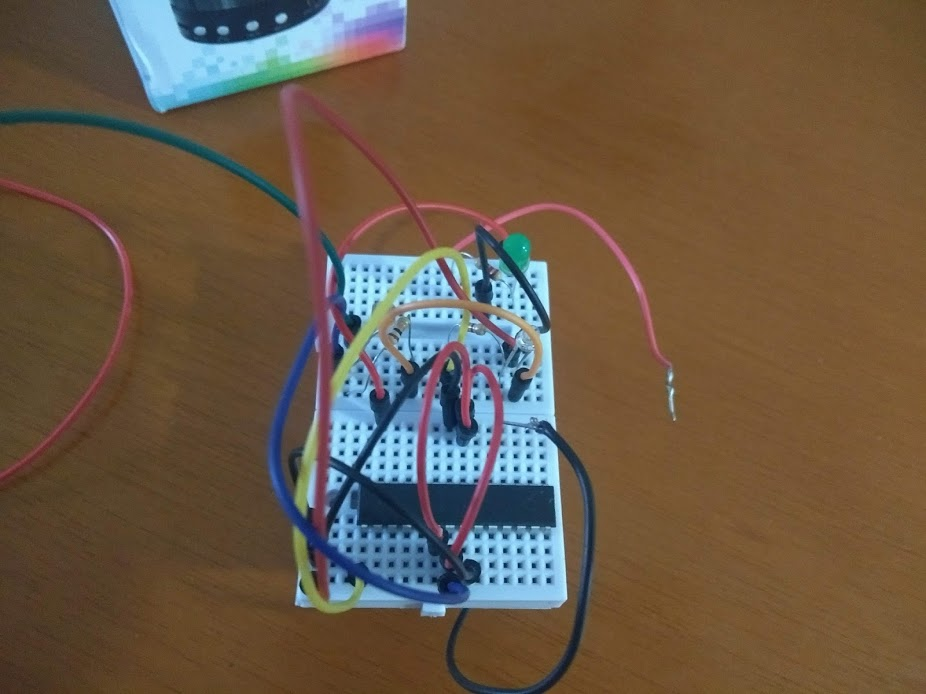
\includegraphics[width=0.6\textwidth]{figuras/indicador.jpg}
            \vspace{\baselineskip} %%% linha em branco para atendender a norma
                \fonte{Autor (2018)}
            \label{fig:led-indicator}
    \end{figure}
    
    Para cada horário, foram realizadas 10 medições por vaga, sendo 10 medidas a cada 10 segundos, resultando em um total de 50 medidas em vagas ocupadas e 50 medidas nas vagas disponíveis. Essas medidas correspondem ao valor cru obtido na leitura do sensor através do conversor AD do microcontrolador, utilizando a referência de tensão externa, afim de evitar que flutuações no nível de tensão da fonte influenciem no resultado. A partir disso, foram estabelecidas estimativas de níveis de intensidade luminosa esperadas para as duas possíveis ocasiões (vaga disponível ou vaga ocupada) em cada horário, baseando-se na média aritmética normalizada das medidas em cada situação. 
    
    \subsubsection{Precisão do sensor}
    Com base nas estimativas de nível de intensidade luminosa, foi avaliada a precisão do sensor em indicar o estado de uma vaga escolhida aleatoriamente no mesmo estacionamento. Assim como nos testes anteriores, foram realizadas 10 medidas por vaga, nos mesmos horários, porém em dias diferentes. 
    
    \begin{figure}[H]
     	    \caption{\label{exepretex} Visão do estacionamento}
            \centering
            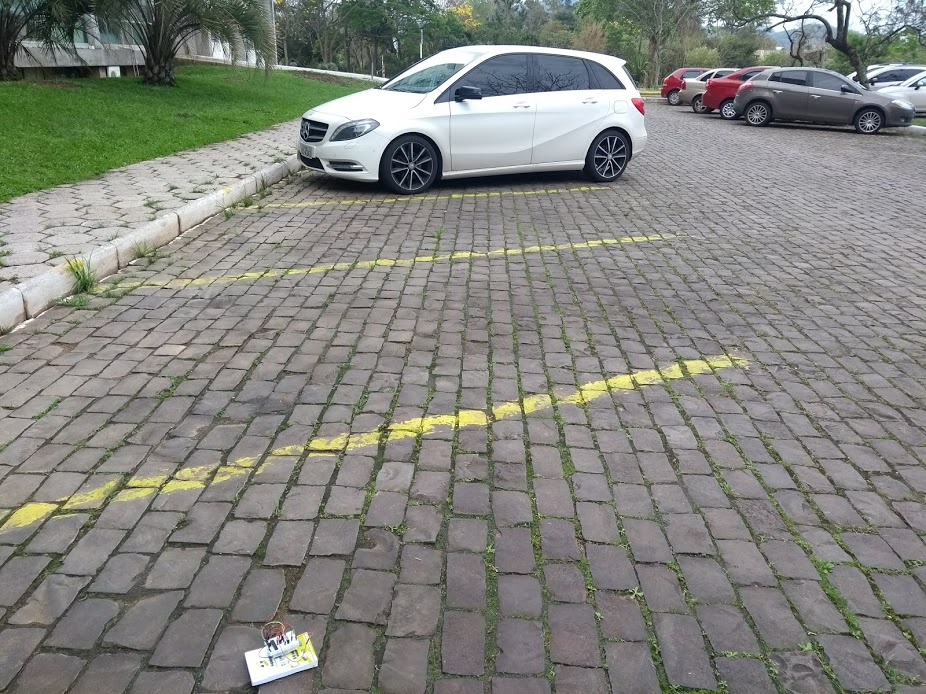
\includegraphics[width=0.6\textwidth]{figuras/estacionamento_visao.jpg}
            \vspace{\baselineskip} %%% linha em branco para atendender a norma
                \fonte{Autor (2018)}
            \label{fig:estac-visao}
    \end{figure}
    
    \begin{figure}[H]
     	    \caption{\label{exepretex} Teste em uma vaga ocupada}
            \centering
            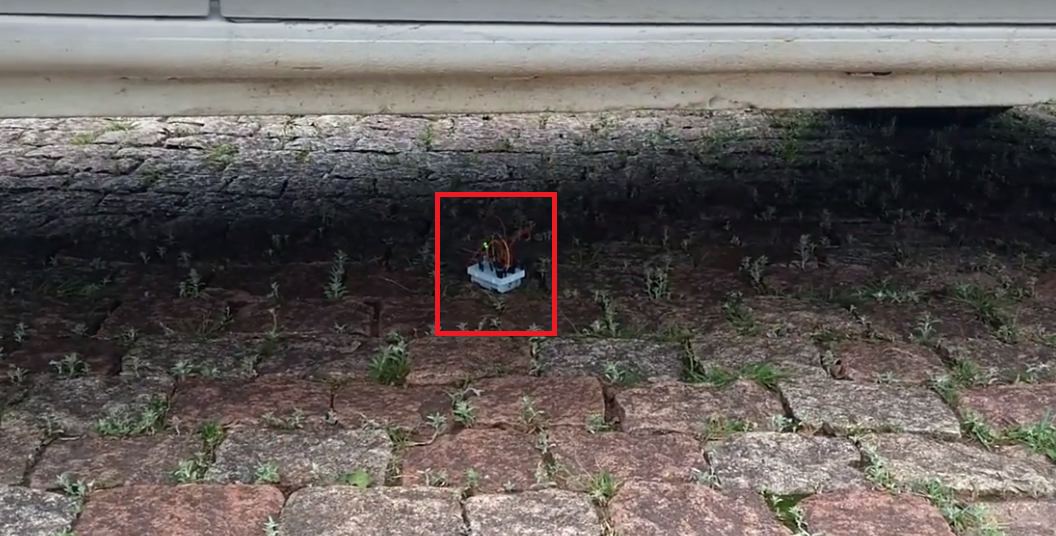
\includegraphics[width=0.6\textwidth]{figuras/ocupada.png}
            \vspace{\baselineskip} %%% linha em branco para atendender a norma
                \fonte{Autor (2018)}
            \label{fig:ocupada}
    \end{figure}
    
    \begin{figure}[H]
     	    \caption{\label{exepretex} Teste em uma vaga disponível}
            \centering
            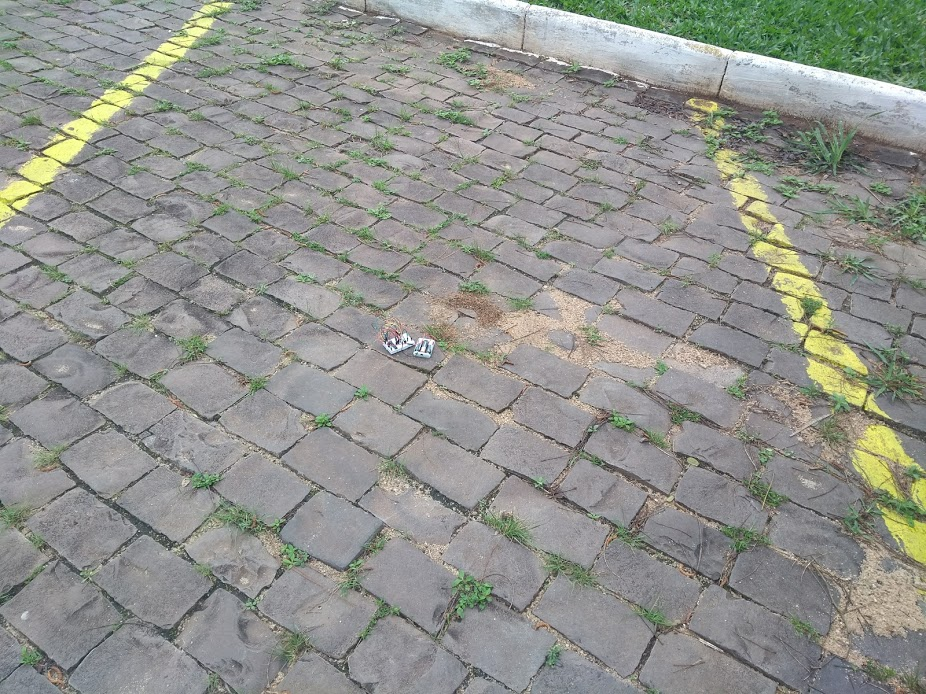
\includegraphics[width=0.6\textwidth]{figuras/disponivel.jpg}
            \vspace{\baselineskip} %%% linha em branco para atendender a norma
                \fonte{Autor (2018)}
            \label{fig:disponivel}
    \end{figure}
    
    \begin{grafico}[H]
     	    \caption{\label{exepretex} Avaliação das medições do LDR ao longo do tempo}
            \centering
            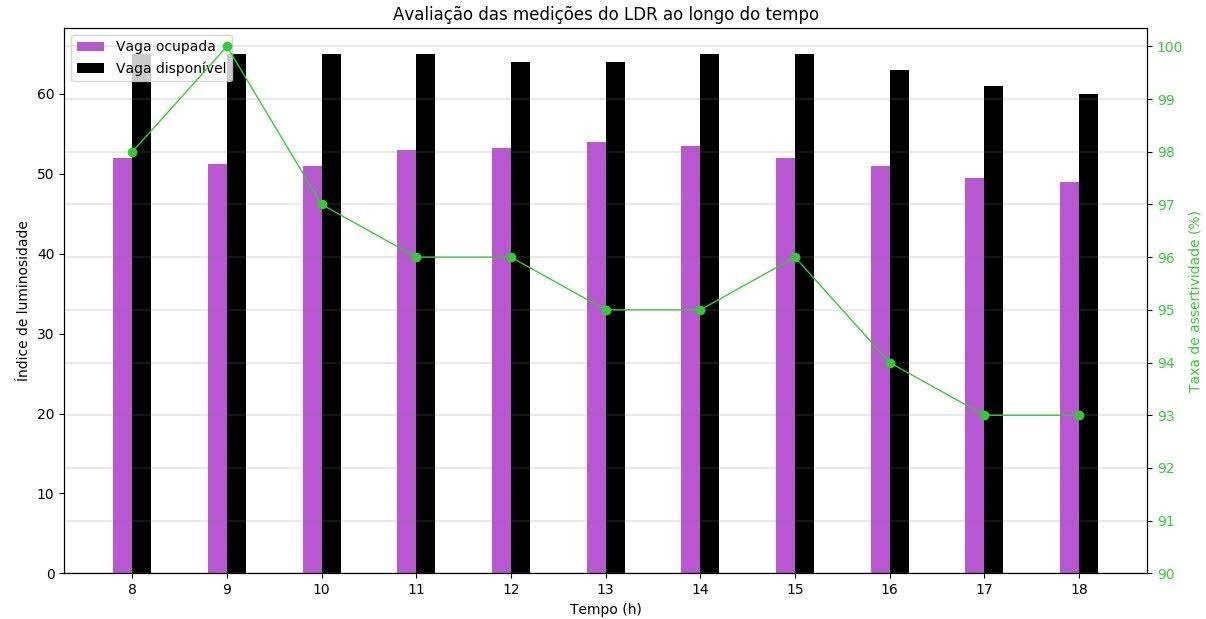
\includegraphics[width=0.8\textwidth]{figuras/ldr_graph.jpg}
            \vspace{\baselineskip} %%% linha em branco para atendender a norma
                \fonte{Autor (2018)}
            \label{graph:ldr-aval}
    \end{grafico}
    
    \subsection{Comunicação entre \textit{sensor node} e \textit{sink node}}
    
    \subsection{Comunicação entre \textit{sink node} e \textit{gateway} LoRa}
    
\section{AVALIAÇÃO DOS RESULTADOS}




\chapter{CONCLUSÕES}
	 

        
% % % % % % % % % % % % % % % % % % % % % % % % % % % % % % % % % % % % % % 
% % % % % % % % % % % % FIM DAS PAGINAS TEXTUAIS % % % % % % % % % % % % % % 
% % % % % % % % % % % % % % % % % % % % % % % % % % % % % % % % % % % % % % 



% % % % % % % % % % % % % % % % % % % % % % % % % % % % % % % % % % % % % % 	
% % % % % % % % % % % % % BIBLIOGRAFIA  % % % % % % % % % % % % % % % % % % 
% % % % % % % % % % % % % % % % % % % % % % % % % % % % % % % % % % % % % % 	

\bibliografia{referencias}  %%%%% BIBLIOGRAFIA -> INCLUIR NAS CHAVES O NOME DO ARQUIVO *.BIB	
	
	
	
% % % % % % % % % % % % % % % % % % % % % % % % % % % % % % % % % % % % % 	
% % % % % % % % % % % % % APENDICES % % % % % % % % % % % % % % % % % % %
% % % % % % % % % % % % % % % % % % % % % % % % % % % % % % % % % % % % % 	
	\apendice %%%% TEXTOS A PARIR DESTE PONTO SERAO CONSIDERADOS APENDICES

\chapter{Demonstração de algo}
        \par Algo como apêndice.  
        \par \begin{figure}[ht]
 	    \caption{\label{exepretex} Fluxograma do \textit{sink node}}
        \centering
        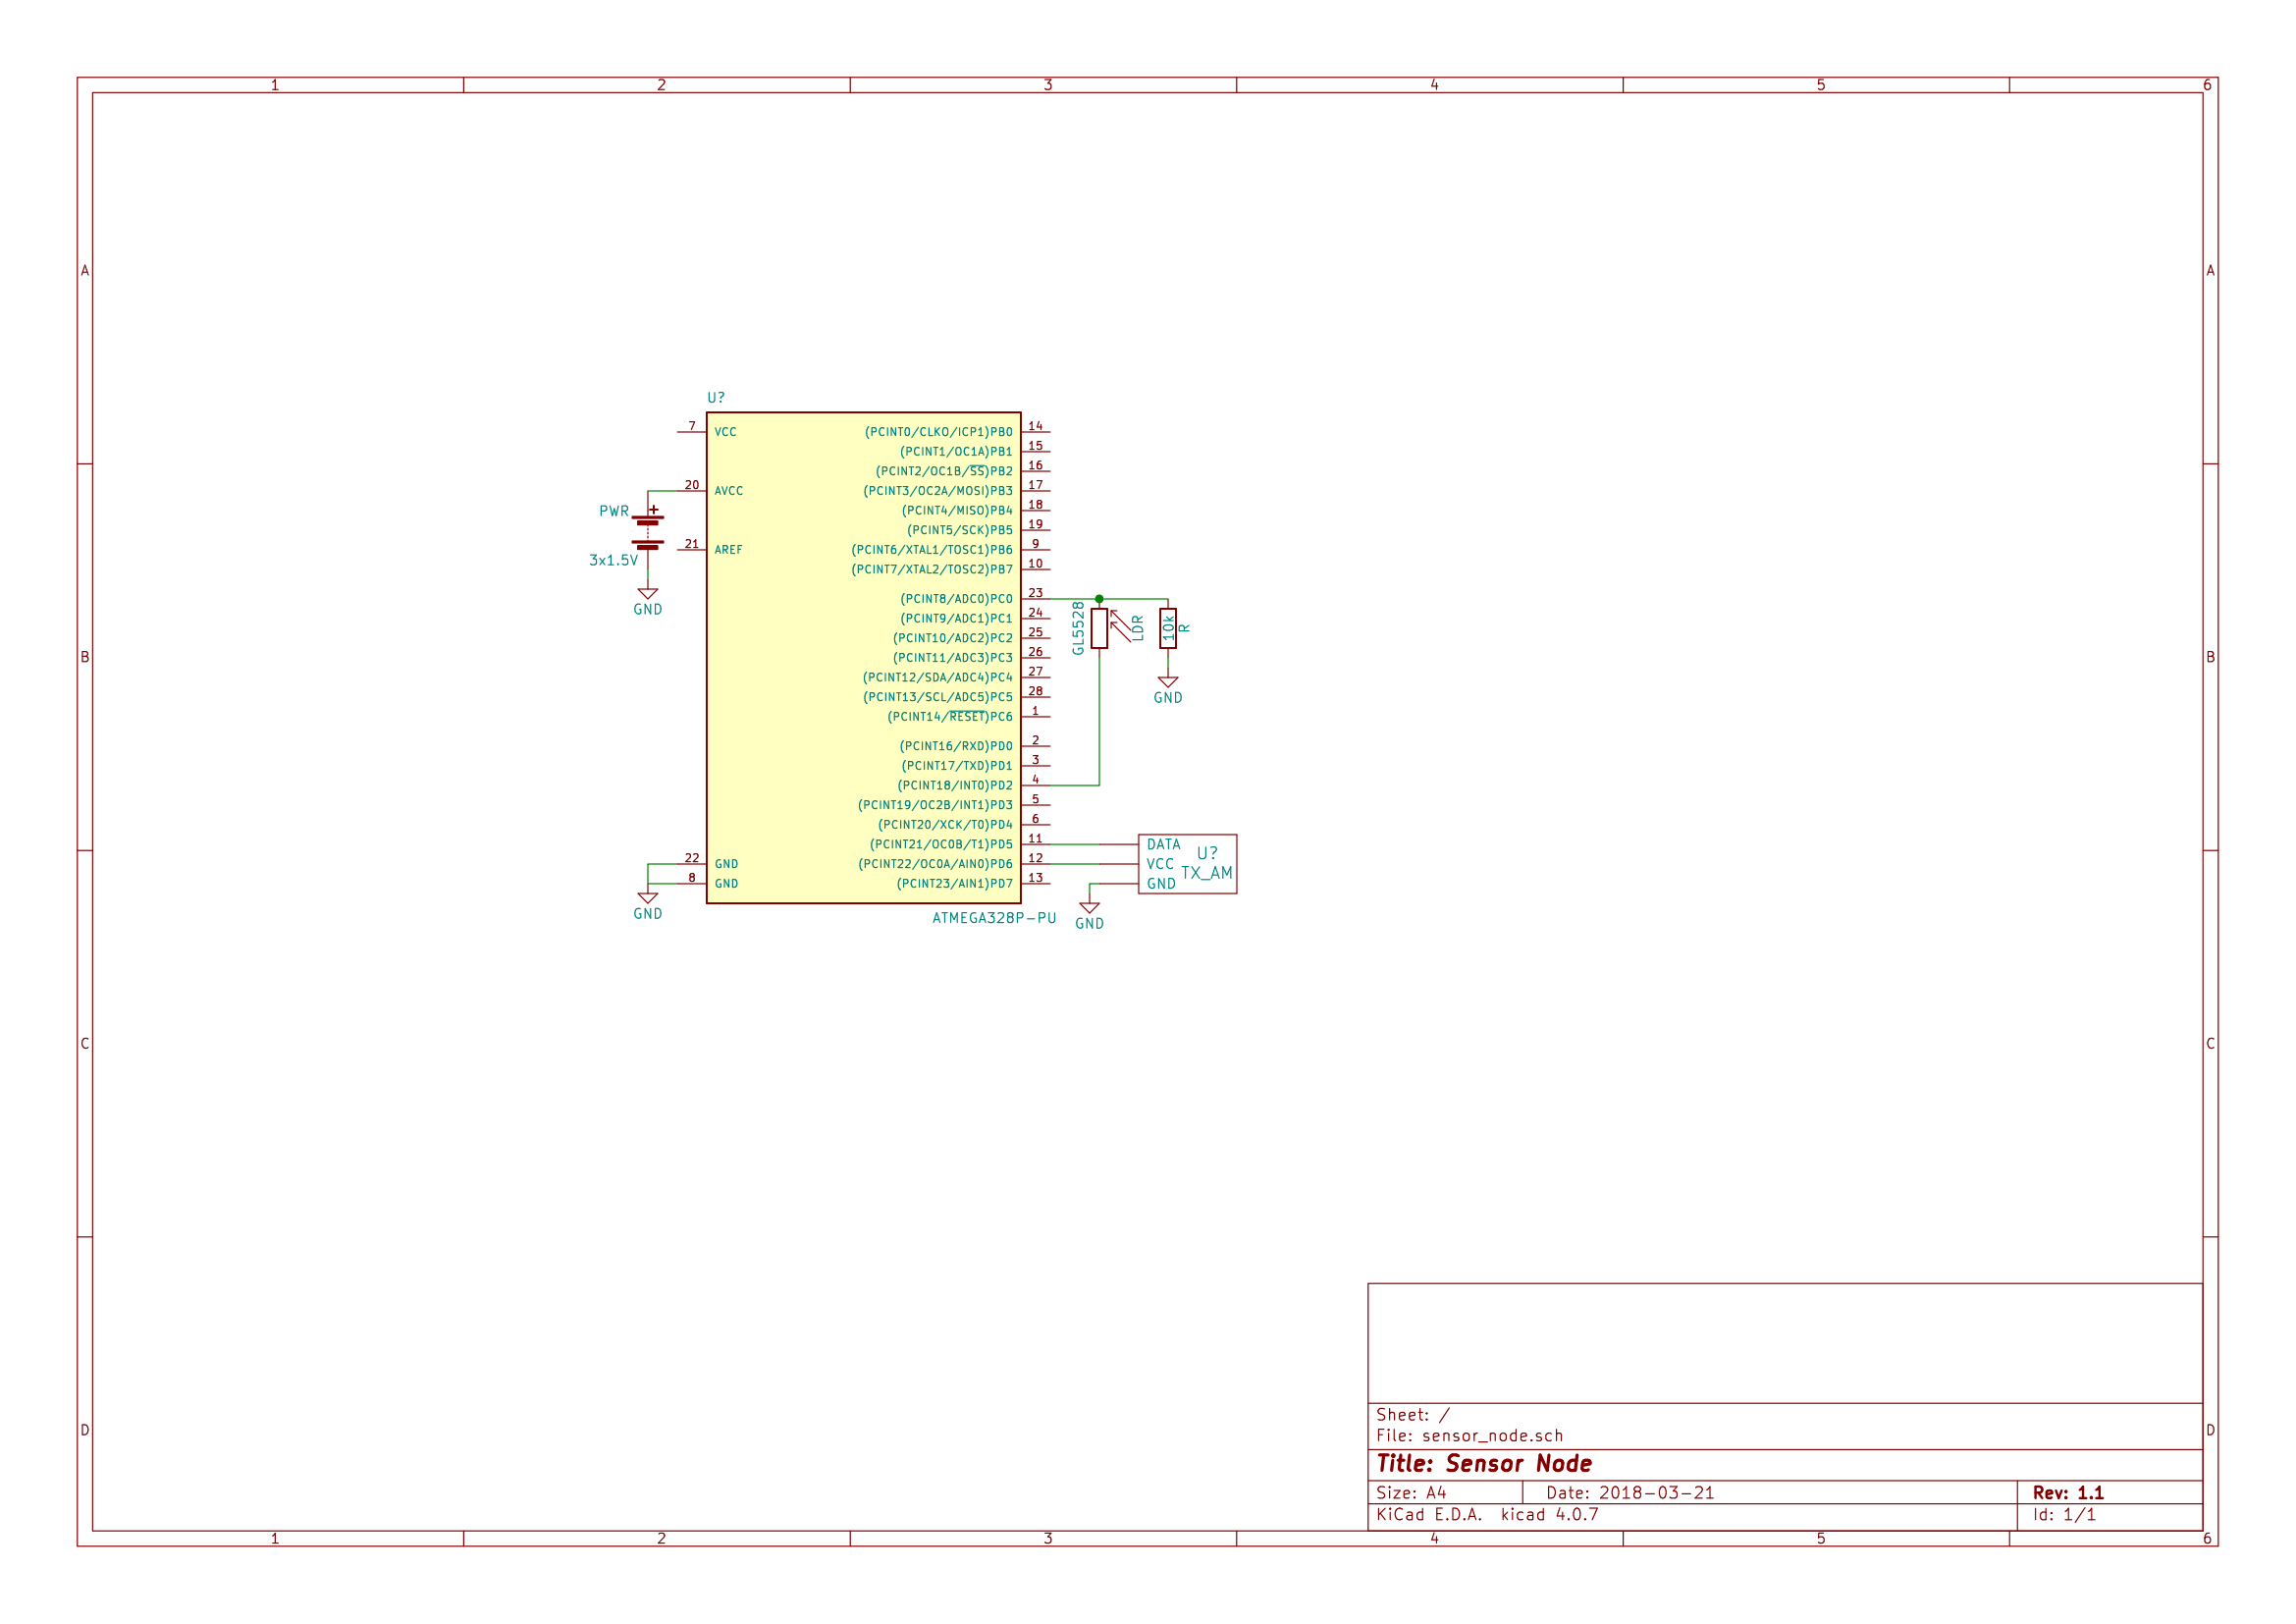
\includegraphics[width=0.6\textwidth]{figuras/sensor_node_v2-1.png}
        \vspace{\baselineskip} %%% linha em branco para atendender a norma
            \fonte{Autor (2018)}
\end{figure}

        
        
        
% % % % % % % % % % % % % % % % % % % % % % % % % % % % % % % % % % % % % % 	
% % % % % % % % % % % % % % % ANEXOS  % % % % % % % % % % % % % % % % % % % 
% % % % % % % % % % % % % % % % % % % % % % % % % % % % % % % % % % % % % % 	
        \anexo    %%%% TEXTOS A PARIR DESTE PONTO SERAO CONSIDERADOS ANEXOS
        
\chapter{Algo interessante que alguém fez}
         \par Algo como anexo.
         
          \begin{verbatim}
	    \begin{ilustracao}[ht]
		\centering
		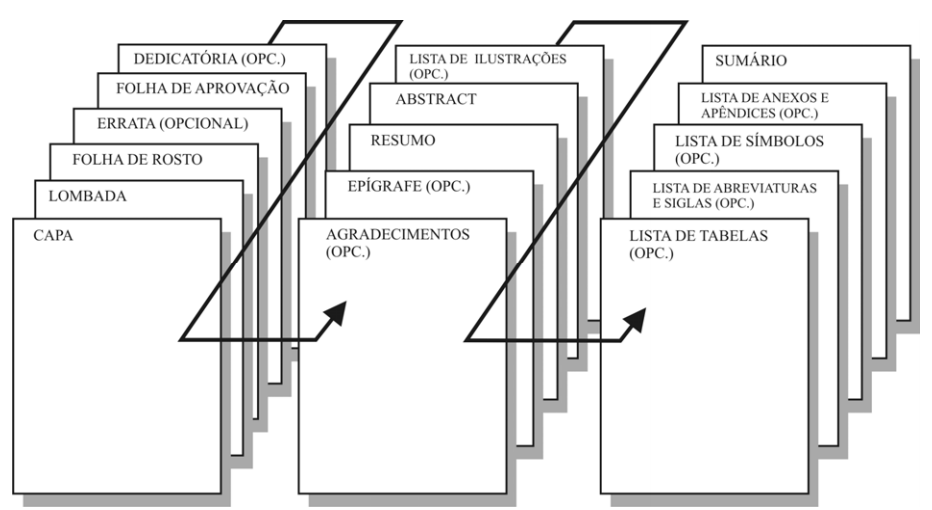
\includegraphics[width=0.6\textwidth]{figuras/pretextuais.png}
		\caption{\label{exepretex} Sequência dos elementros pré-testuais da MDT-UFSM}
		\vspace{\baselineskip} %%% linha em branco para atendender a norma
		\fonte{Adaptado de \citeonline{man:MDTUFSM2012}.}
	    \end{ilustracao}
         \end{verbatim}
         
         \begin{grafico}[ht]
     	    \caption{\label{exepretex1} Sequência dos elementros pré-testuais da MDT-UFSM}
	    \centering
	    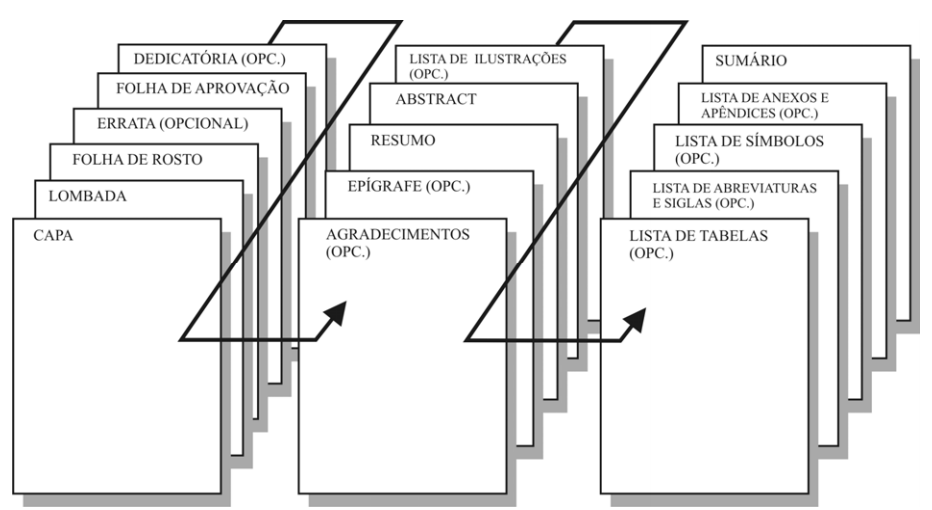
\includegraphics[width=0.6\textwidth]{figuras/pretextuais.png}
	    \vspace{\baselineskip} %%% linha em branco para atendender a norma
            \fonte{Adaptado de \citeonline{man:MDTUFSM2012}.}
         \end{grafico}
         
         
         \section*{Teste de seção dentro do anexo}


\end{document}

